\documentclass[12pt,oneside]{book}
\pagestyle{headings}

% Note that the line below could be modified to suit a
% particular system since the "geometry" package behaves
% differently in Unix, Windows and Mac, especially for the
% top margins.
% Adjust the parameter "top" (measuring the height of the
% space allocated to a header) and "headsep" (measuring
% the distance from the bottom of the header to the
% first line of text.
\usepackage[top=1.3in,left=1.5in,bottom=1in,right=1in,headsep=0.5in]{geometry}

\usepackage{setspace}
\onehalfspacing
%\doublespacing

% Headers and footers for thesis
\usepackage{fancyhdr}

\markboth{}{}
\newcommand\startchapter[1]{\chapter{#1}\thispagestyle{myheadings}}
\newcommand\startappendix[1]{\chapter{#1}\thispagestyle{myheadings}}
\newcommand\startfirstchapter[1]{\chapter{#1}}

% Manual addition of section to Table of Contents
\newcommand\TOCadd[1]{\newpage\phantomsection\addcontentsline{toc}{chapter}{#1}}

% Float Customization
\renewcommand{\floatpagefraction}{0.01}

% Customization of Tables of Contents and List of Figures/Tables
\usepackage{tocloft}
\renewcommand\cfttabpresnum{Table\ }
\renewcommand\cfttabnumwidth{0.75in}
\renewcommand\cftfigpresnum{Figure\ }
\renewcommand\cftfignumwidth{0.80in}
\newcommand{\HRule}{\rule{\linewidth}{0.5mm}}


% Long Table and decimal aligned columns
\usepackage{dcolumn}
\usepackage{longtable}

% Mathematics support
\usepackage{amsmath}
\usepackage{amsthm}
\usepackage{amssymb}


% Text Control
\usepackage{xspace}
\usepackage{textcase}

% Graphics
\usepackage{wasysym}
\usepackage{graphics}
\usepackage{graphicx}   % A package to allow insertion of
                        % external image files


\usepackage{cite}
\usepackage[acronym]{glossaries}
\usepackage{nomencl}
%\loadglsentries{Utils/Glossary}
\makenomenclature
\renewcommand{\nomname}{List of Symbols}

\newcommand{\Xilinx}{\textit{Xilinx}~}
%%%%%%%%%%%%%%%%%%%%%%%%%%%%%%%%%%%%%%%%%%%%%%%%%%%%%%%%%
%To compile glossary and acronyms run following sequence under Tools
%Commands -> pdfLatex
%User -> MakeGlossaries
%Commands -> Make Index
%Commands -> pdfLatex
%Build
%%%%%%%%%%%%%%%%%%%%%%%%Acronyms%%%%%%%%%%%%%%%%%%%%%%%%%
\newacronym{FPGA}{FPGA}{Field Programmable Gate-Array}
\newacronym{FPGAs}{FPGA}{Field Programmable Gate-Arrays}
\newacronym{CL}{CL}{Configurable Logic}
\newacronym{ASIC}{ASIC}{Application Specific Integrated Circuit}
\newacronym{HDL}{HDL}{Hardware Description Language}
\newacronym{ISE}{ISE}{Integrated Synthesis Environment}
\newacronym{IOB}{IOB}{Input-Output Blocks}
\newacronym{CLB}{CLB}{Configurable Logic Block}
\newacronym{LUT}{LUT}{Look-up Table}
\newacronym{IR}{IR}{Interconnect Resources}
\newacronym{SM}{SM}{Switching Matrix}
\newacronym{PIP}{PIP}{Programmable-Interconnect-Points}
\newacronym{XDL}{XDL}{\Xilinx Design Language}
\newacronym{RDB}{RDB}{Readback File}
\newacronym{MSD}{MSD}{The mask file used to hide undesirable configuration information}
\newacronym{DFF}{DFF}{D Flip-Flop}
\newacronym{TCL}{TCL}{Tool Command Line}
\newacronym{JTAG}{JTAG}{Joint Test Action Group}
\newacronym{SRL}{SRL}{Shift Right Left Module}
\newacronym{RAM}{RAM}{Random Access Memory}
\newacronym{LL}{LL}{Logic Allocation File}
\newacronym{RBB}{RBB}{Repeatable Building Blocks}
\newacronym{RBA}{RBA}{Readback ASCII}
\newacronym{RTL}{RTL}{Registry Transfer Level}
\newacronym{TV}{TV}{Test Vectors}
\newacronym{XOR}{XOR}{Exclusive OR}
\newacronym{XNOR}{XNOR}{Exclusive NOR}
\newacronym{UUT}{UUT}{Unit Under Test}
\newacronym{PROM}{PROM}{Programmable Read-Only Memory}
\newacronym{GUI}{GUI}{Graphical User-Interface}
\newacronym{EDIF}{EDIF}{Electronic Data Interchange Format}
\newacronym{NCF}{NCF}{Netlist Constraints File}
\newacronym{UI}{UI}{User-Interface}
\newacronym{DCM}{DCM}{Digital Clock Managers}
\newacronym{ROM}{ROM}{Read-Only Memory}
\newacronym{BEL}{BEL}{Basic Element}
\newacronym{UCF}{UCF}{User Constraint File}
\newacronym{API}{API}{Application Programming Interface}
\newacronym{IO}{IO}{Input-Output}
\newacronym{BRAM}{BRAM}{Block RAM}
\newacronym{SRAM}{SRAM}{Static RAM}
\newacronym{CMD}{CMD}{Command Register}
\newacronym{WCFG}{WCFG}{CMD Write Packet Data}
\newacronym{MSK}{MSK}{Readback Mask File}
\newacronym{appName}{\textit{F-TRAP}}{\acrshort{FPGA} Trojan Recognition and Parsing}
\newacronym{FLR}{FLR}{Frame Length Register}
\newacronym{IC}{IC}{Integrated Circuit}
\newacronym{ICs}{IC}{Integrated Circuits}
\newacronym{PLD}{PLD}{Programmable Logic Device}
\newacronym{PLDs}{PLD}{Programmable Logic Devices}
\newacronym{ERAI}{ERAI}{Electronic Resellers Association International}
%%%%%%%%%%%%%%%%%%%%%%%%Glossary Entries%%%%%%%%%%%%%%%%%
\newglossaryentry{log}{name={log},description={A log file generated by XST}}
\newglossaryentry{Bitstream}{name={Bitstream},description={The sequence of one and zeroes which makes up the configuration data}}
\newglossaryentry{Bit}{name={Bit},description={The binary file containing the configuration data for the implementation}}
\newglossaryentry{Vivado}{name={Vivado},description={The Integrated Development Environment Used Exclusively for 7-series FPGAs}}
\newglossaryentry{Xilinx}{name={\Xilinx},description={The largest producer of FPGAs used exclusively for this proposal}}
\newglossaryentry{Readback}{name={Readback},description={A feature in all \Xilinx FPGAs where by the current state of the \gls{gateArray} is stored in the configuration memory to be read by the user via the JTAG port}}
\newglossaryentry{SelectMap}{name={SelectMap},description={A \Xilinx device configuration mode which allows for the programming of multiple devices in parallel}}
\newglossaryentry{golden}{name={Golden},description={The clean, untampered version of the synthesis files generated by XST}}
\newglossaryentry{target}{name={Target},description={The generated files from devices received from the third-party fabrication house}}
\newglossaryentry{Library}{name={\textit{Library}},description={The list of absolute addresses for all components in a \gls{gateArray}}}
\newglossaryentry{NGC}{name={NGC},description={The NGC file is a netlist that contains both logical design data and constraints. The NGC file takes the place of both \acrfull{EDIF} and \acrfull{NCF} files}}
\newglossaryentry{Plan Ahead}{name={Plan Ahead},description={Software provided by \Xilinx for RTL to bitstream design flow management}}
\newglossaryentry{RAM16}{name={RAM16},description={\acrshort{LUT} used as a 16x1 memory unit}}
\newglossaryentry{SRL16}{name={SRL16},description={\acrshort{LUT} used as a 16-bit shift register}}
\newglossaryentry{SLICEM}{name={SLICEM},description={A component of a \acrshort{CLB} in the Spartan-3E family of \acrshort{FPGA}s capable of both logic and memory functions}}
\newglossaryentry{SLICEL}{name={SLICEL},description={A component of a \acrshort{CLB} in the Spartan-3E family of \acrshort{FPGA}s capable of only logic functions}}
\newglossaryentry{sch2hdl}{name={sch2hdl},description={A \gls{Xilinx} tool used to convert schematic designs to \gls{HDL}}}
\newglossaryentry{XST}{name={XST},description={\gls{Xilinx} Synthesis Tools}}
\newglossaryentry{ngdbuild}{name={ngdbuild},description={A \gls{Xilinx} tool used to build a NETLIST}}
\newglossaryentry{MAP}{name={MAP},description={A \gls{Xilinx} tool used to calculate the optimal routing map for the implementation fo the design}}
\newglossaryentry{PAR}{name={PAR},description={A \gls{Xilinx} tool used to place and route the design in the specific device}}
\newglossaryentry{trce}{name={trce},description={A \gls{Xilinx} tool used to perform timing of routing traces}}
\newglossaryentry{Bitgen}{name={Bitgen},description={A \gls{Xilinx} tool used to generate the final configuration \gls{Bitstream}}}
\newglossaryentry{thread}{name={thread},description={The smallest sequence of programmed instructions that can be managed independently by a scheduler, which is typically a part of the operating system.}}
\newglossaryentry{Group}{name={Group},description={A collection of columns of 1-bit wide components in an FPGA}}
\newglossaryentry{FragementMatrix}{name={Fragement Matrix},description={A conceptual interpretation of the architecture of an FPGA where by it is imagined as a matrix of 1-bit configurable components}}
\newglossaryentry{QT}{name={QT},description={ a cross-platform application framework that is widely used for developing application software that can be run on various software and hardware platforms. It provides easy to use \acrshort{UI} design tools and features used for this project.~\cite{QT}}}
\newglossaryentry{Boost}{name={Boost},description={ a set of libraries for the C++ programming language that provide support for tasks and structures such as linear algebra, pseudorandom number generation, multithreading, image processing, regular expressions, and unit testing.~\cite{boostLibrary}}}
\newglossaryentry{winAPI}{name={Windows \gls{API}},description={Windows API or WinAPI is a core set of Microsoft's \acrshort{API}s available within the Windows Operating System. It provides basic \acrshort{UI}, Environment handling, data access and storage utilities and more.~\cite{windowsAPI}}}
\newglossaryentry{Fragment}{name={Fragment},description={A 1-bit configurable component of an FPGA. Fragments do not exist however they are used as a conceptual aid to improve understanding of configuration process.}}
\newglossaryentry{gateArray}{name={Gate Array},description={The primary structure of an \gls{FPGA} device. Composed of a regular arrangement of logic gates.}}
\makeglossaries


\begin{document}

% Front Matter
\input frontmatter/fm

\newpage

	\startfirstchapter{Introduction}
\label{chapter:introduction}
The term \textit{Trojan Horse} or \textit{Trojan} has become a modern metaphor for a deception where by an unsuspecting victim welcomes a foe into an otherwise safe environment~\cite{searchForTrojanWar}.
Though modern civilization rarely has need for large walls we are similarly surrounded.
Not by stone and mortar but by the technology we so heavily rely on.
These days it is more common to come across a piece of equipment with some form of computer in it than without.
They provide us entertainment, education, security, monitor our health, grow our food and more.
Our reliance make us susceptible to their compromise.
Since the dawn of the computer we have dealt with software threats.
We are almost as good at protecting ourselves against them as attackers are at making them.
In recent years a new incarnation of electronic danger has emerged; in hardware.
In this new arena of attack and defend those who seek to defend are far behind.

\section{Motivation}
In the summer of 2007 an Israeli military action referred to as Operation Orchard commenced.
A group of F-15I Ra'am fighter jets from the Israeli Air Force 69th Squadron took off to attack a suspected nuclear reactor in neighboring Syria~\cite{stoppingHTsIEEESpectrum}.
In the flight path was a Syrian radar station which boasted ``state-of-the-art'' aircraft detection and neutralization technology. 
The Israeli war planes were able to approach and destroy the installation undetected.
Though never proven it is commonly accepted that the detection mechanism was deactivated by a back-door circuit inserted into the radar system.
In 2011 over 1300 cases of modified \acrshort{IC}s were reported to the \acrfull{ERAI}; the occurrence of such cases has since been going up~\cite{counterfeitIEEESpectrum}.
\acrfull{ICs} are a large part of modern life yet it is easy to forget that they drive virtually every piece of technology used today.
Ensuring that their \acrshort{IC}s run our devices as expected is vital in the digital era.
Since their discovery there has been concerted effort to detect these modifications but the innate complexity of \acrshort{IC}s makes it difficult~\cite{hardwareTrojanSurvey2015}.
These modifications are commonly known as hardware trojans.

One of the most commonly attempted trojan detection techniques is to apply a series of inputs and look to see if the outputs are as expected.
This is known as Functional testing or Test Vectoring \cite{kSubset,monteCarloTestPattern,towardsDetectionMethodology}.
This method has been shown to provide some success but is commonly beaten by attackers.
Another common strategy is to search for side effects of modified circuits; these methods are referred to as ``side-channel'' analysis methods.
Such side effects include, changes to power consumption, temperature differences, radiation differences and more~\cite{sideChannelObfuscation, postLayout, controllableSleepTransistors, pcaAlgorithm}.
Again, these methods provide varying success but face a lot of difficulty.
Trojans and detection methods alike are new.
The work in this field has only seen progress in the last few decades.
The results of this work are still primarily buried in academic publications in various locations, in various formats.
The discovery of what has already been achieved and what still needs to be done in this field is arduous 

\acrshort{IC} designs for \acrfull{FPGAs} are made using a software language.
The design is then converted to a binary file called a configuration \gls{Bitstream} which is then downloaded onto the device; this process is known as synthesizing the design.
There have been many attempts to develop mechanisms and techniques to determine whether a malicious user has tampered with the design via test vectoring or side-channel analysis.
As of yet there has been little effort to directly analyze the configuration \gls{Bitstream}.


\section{Contributions}
The goal of this work is two-fold.
First, to prove that analysis of the configuration \gls{Bitstream} is the most powerful means of detecting trojans in \acrshort{FPGA}s.
To do so, an application was developed which parses and analyzes the \gls{Bitstream}, detects the presence of trojans and provides an astute description of the modification.
Secondly, to provide a centralized place for researchers to review and analyze discovered trojans.
A website was developed which provides the automation of useful analysis techniques as well as a database, yet to be populated, of all known trojans and detection methods. 

The contributions of this work can be said to be:
\begin{enumerate}
	\item Proof that though \acrshort{FPGA} manufacturers hide the intimate details of the configuration \gls{Bitstream} it is the most viable means of trojan detection and analysis. 
	\item Proof of concept for a new method of detecting and analyzing trojans.
	\item Develop a software application which automates the described methodology.
	\item Develop a database structure to house all known trojans and detection methods
	\item A user friendly web site to interact and access the trojan/detection method database.
\end{enumerate}
\section{Organization}
This enclosing section presents a map of this work and a short description of each chapter.
Chapter 2 provides some background information on trojans themselves and introduces the descriptive taxonomy used.
Chapter 3 introduces the new detection and analysis methodology.
It gives a brief overview of \acrshort{FPGA} architecture and configuration, describes the analysis process of the \gls{Bitstream}, introduces \textit{Component Mapping}, and discusses how the taxonomic attributes are extracted.
Chapter 4 presents an online 
%Chapter 4 discusses the software implementation which has been named \Name.
It discusses the technologies used and why they were chosen, presents the \acrlong{UI} and discusses its operating procedure.
Chapter 5 presents the results of experimentation done using three \acrshort{FPGA}-trojan benchmarks
These benchmarks were specifically chosen to demonstrate that the application works as expected and is easy to use.
Finally, chapter 6 concludes this work and restates its contributions.
	\startchapter{Hardware Trojans}
\label{chapter:hardwareTrojans}

\newlength{\savedunitlength}
\setlength{\unitlength}{2em}
\section{Background} \label{sec:trojanBackGround}
\acrfull{ICs} are continuously decreasing in size whilst increasing in complexity.
These trends require ever more people and sophisticated means of manufacture which in turn creates security vulnerabilities.
Products developed by semiconductor companies generally compromised in one of two ways.
First, due to the complexity it is rare for a product to be managed within a single company.
Frequently, steps in the production-chain are outsourced.
It is within these 'third-party' contributors that products can be maliciously modified.
Secondly, for various reasons, employees of trusted contributors have been known to make modifications.~\cite{trojanSurvey2014}
These modifications are known as hardware Trojans.
\acrshort{IC}s are an integral part of every facet of the modern world.
Proper application of a Trojan can provide information, control of mechanical systems, surveillance and more to an unauthorized party.


\section{Topology} \label{sec:topology}
The discussion, detection and evaluation of hardware trojans requires a comprehensive means of description.
Several hardware trojan taxonomies have been proposed~\cite{taxonomy1, taxonomy2, taxonomy3, taxonomy4}.
In~\cite{taxonomy1}, trojans were organized based solely on their activation mechanisms.
A taxonomy based on the location, activation and action of a trojan was presented in \cite{taxonomy2}, \cite{taxonomy3}.
However, these approaches do not consider the manufacturing process.
Another taxonomy was proposed in~\cite{taxonomy4} which employs five categories: insertion, abstraction, activation, effect, and location.
While this is more extensive than previous approaches, it fails to account for the physical characteristics of a trojan.
An additional taxonomy was proposed in~\cite{samerAttribute} which considers all attributes a hardware trojan may posses.
This taxonomy is the most comprehensive and was selected as the means of description for this work.
\begin{figure}
	\centering
	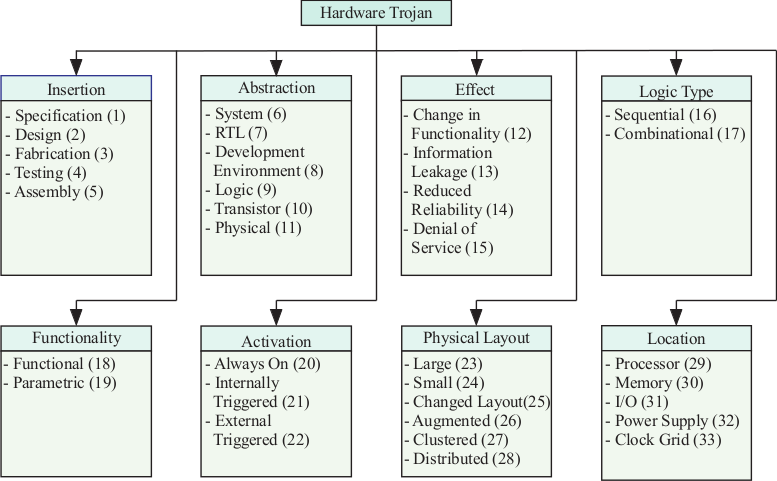
\includegraphics[width=1.0\linewidth]{figures/HW_trojan}
	\caption{The thirty-three attributes of the hardware trojan taxonomy in~\cite{samerAttribute}.}
	\label{fig:HW_trojan}
\end{figure}
It is comprised of thirty-three attributes organized into eight categories as shown in Fig.~\ref{fig:HW_trojan}.
These categories can be arranged into the following four levels as indicated in Fig.~\ref{fig:trojan_life_cycle}.
\begin{enumerate}
	\item The \textbf{insertion} (chip life-cycle) level/category comprises the attributes pertaining to the IC production stages.
	\item The \textbf{abstraction} level/category corresponds to where in the IC abstraction the trojan is introduced.
	\item The \textbf{properties} level comprises the behavior and physical characteristics of the trojan.
	\item The \textbf{location} level/category corresponds to the location of the trojan in the IC.
\end{enumerate}
The properties level consists of the following categories.
\begin{itemize}
	\item The \textbf{effect} describes the disruption or effect a trojan has on the system.
	\item The \textbf{logic type} is the circuit logic that triggers the trojan, either combinational or sequential.
	\item The \textbf{functionality} differentiates between trojans which are functional or parametric.
	\item The \textbf{activation} differentiates between trojans which are always on or triggered.
	\item The \textbf{layout} is based on the physical characteristics of the trojan.
\end{itemize}
\begin{figure}
	\centering
	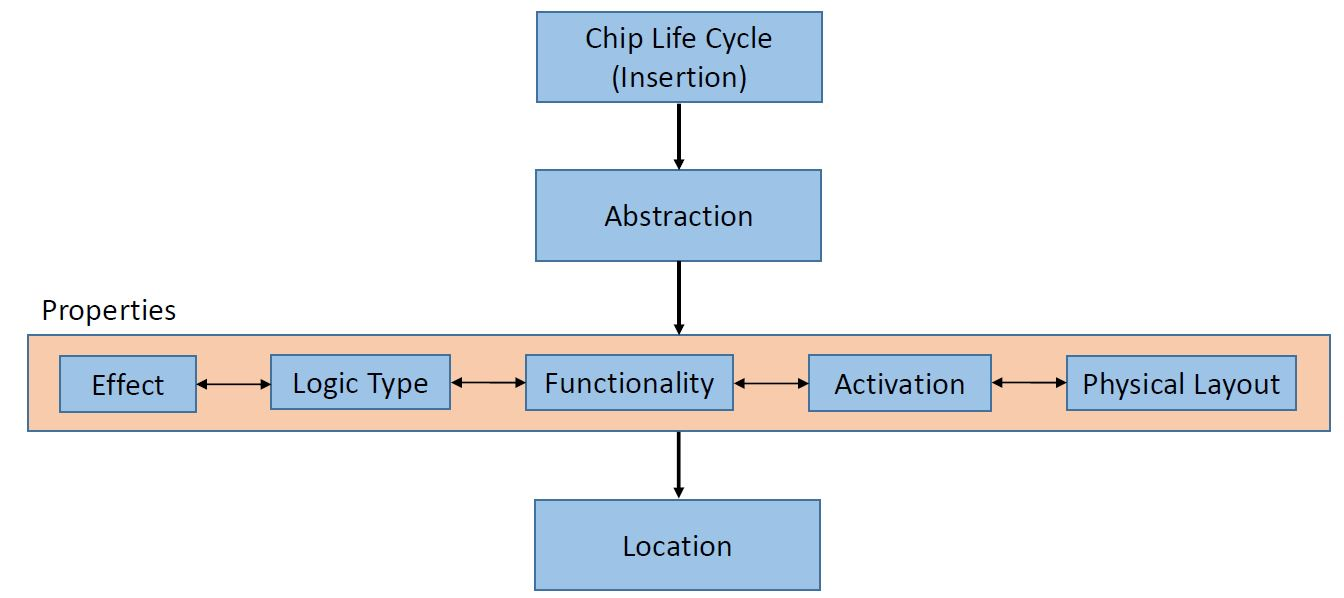
\includegraphics[width=0.8\linewidth]{figures/trojan_life_cycle}
	\caption{The hardware trojan levels \cite{samerAttribute}.}
	\label{fig:trojan_life_cycle}
\end{figure}

\begin{table*}
	\[
	\newcommand\scalemath[2]{\scalebox{#1}{\mbox{\ensuremath{\displaystyle #2}}}}
	\mathbf{R} =
	\left[
	\scalemath{0.5}{
		\begin{array}{l||c|c|c|c|c||c|c|c|c|c|c||c|c|c|c|c|c|c|c|c|c|c|c|c|c|c|c|c||c|c|c|c|c}
		A & 1$~$ & 2$~$  & 3$~$ & 4$~$& 5$~$ & 6$~$  & 7$~$ & 8$~$ & 9$~$ & 10  & 11 & 12& 13 & 14  & 15 & 16& 17 & 18  & 19 & 20& 21 & 22  & 23 & 24& 25 & 26  & 27 & 28 & 29 &30 & 31 & 32 & 33\\ \hline \hline
		1 & 0 & 1 & 0 & 0 & 0 & 1 & 0 & 0 & 0 & 0 & 0 &  &  &  &  &  &  &  &  &  &  &  &  &  &  &  &  &   &  &  &  &  &  \\ \hline
		2 & 0 & 0 & 1 & 0 & 0 & 0 & 1 & 0 & 0 & 0 & 0 &  &  &  &  &  &  &  &  &  &  &  &  &  &  &  &  & &  &  &  &  &   \\ \hline
		3 & 0 & 0 & 0 & 1 & 0 & 0 & 0 & 0 & 0 & 0 & 1 &  &  &  &  &  &  &  &  &  &  &  &  &  &  &  &  & &  &  &  &  &   \\  \hline
		4 & 0 & 0 & 0 & 0 & 1 & 1 & 0 & 0 & 1 & 0 & 0 &  &  &  &  &  &  &  &  &  &  &  &  &  &  &  &  &&  &  &  &  &    \\  \hline
		5 & 0 & 0 & 0 & 0 & 0 & 1 & 0 & 0 & 0 & 0 & 0 &  &  &  &  &  &  &  &  &  &  &  &  &  &  &  &  &  &  &  &  &  &  \\  \hline \hline
		6 &  &  &  &  &  & 0 & 1 & 0 & 0 & 0 & 0 &1 & 1 & 0 & 1 & 0 & 0 & 1 & 1 & 1 & 0 & 0 & 0 & 0 & 0 & 0 & 0 & 0  &  &  &  &  &  \\ \hline
		7 &  &  &  &  &  & 0 & 0 & 1 & 0 & 0 & 0 &1 & 0 & 0 & 1 & 1 & 1 & 1 & 0 & 1 & 1 & 1 & 1 & 1 & 0 & 0 & 0 & 0  &  &  &  &  &   \\ \hline
		8 &  &  &  &  &  & 0 & 0 & 0 & 1 & 0 & 0 &1 & 0 & 0 & 1 & 1 & 1 & 1 & 0 & 1 & 1 & 1 & 1 & 1 & 1 & 1 & 1 & 1  &  &  &  &  &   \\ \hline
		9 &  &  &  &  &  & 0 & 0 & 0 & 0 & 1 & 0 & 1 & 0 & 0 & 1 & 1 & 1 & 1 & 0 & 1 & 1 & 1 & 0 & 0 & 0 & 0 & 0 & 0 &  &  &  &  &    \\ \hline
		10 &  &  &  &  &  & 0 & 0 & 0 & 0 & 0 & 1 & 1 & 0 & 1 & 0 & 0 & 1 & 1 & 1 & 1 & 0 & 0 & 0 & 1 & 0 & 1 & 1 & 0  &  &  &  &  &  \\  \hline
		11 &  &  &  &  &  & 0 & 0 & 0 & 0 & 0 & 0 &1 & 1 & 1 & 0 & 0 & 0 & 1 & 1 & 1 & 0 & 0 & 1 & 1 & 1 & 1 & 1 & 1  &  &  &  &  &    \\  \hline \hline
		12 & &  &  &  &  &  &  &  &  &  &  & 0 & 0 & 0 & 0 & 1 & 1 & 1 & 0 & 1 & 1 & 1 & 1 & 1 & 1 & 1 & 1 & 1&1 & 1 & 1 & 1 & 1 \\ \hline
		13 & &  &  &  &  &  &  &  &  &  &  &0 & 0 & 0 & 0 & 0 & 1 & 0 & 1 & 1 & 0 & 1 & 0 & 1 & 0 & 1 & 1 & 1&1 & 1 & 1 & 1 & 1 \\ \hline
		14 &&  &  &  &  &  &  &  &  &  &  & 0 & 0 & 0 & 0 & 0 & 0 & 0 & 1 & 1 & 0 & 0 & 0 & 1 & 0 & 1 & 1 & 1&1 & 1 & 1 & 1 & 1 \\ \hline
		15 & &  &  &  &  &  &  &  &  &  &  &0 & 0 & 0 & 0 & 1 & 1 & 1 & 0 & 1 & 1 & 1 & 1 & 1 & 1 & 1 & 1 & 1&1 & 0 & 1 & 1 & 1 \\ \hline
		16 & &  &  &  &  &  &  &  &  &  &  &1 & 0 & 0 & 1 & 0 & 0 & 1 & 0 & 0 & 1 & 1 & 1 & 0 & 1 & 1 & 1 & 1&1 & 1 & 1 & 1 & 1 \\ \hline
		17 & &  &  &  &  &  &  &  &  &  &  &1 & 1 & 0 & 1 & 0 &0 & 1 & 0 & 1 & 1 & 1 & 1 & 1 & 1 & 1 & 1 & 1&1 & 1 & 1 & 1 & 1 \\ \hline
		18 & &  &  &  &  &  &  &  &  &  &  &1 & 0 & 0 & 1 & 1 & 1 & 0 & 0 & 1 & 1 & 1 & 1 & 1 & 1 & 1 & 1 & 1&1 & 1 & 1 & 1 & 1 \\ \hline
		19 & &  &  &  &  &  &  &  &  &  &  &0 & 1 & 1 & 0 & 0 & 0 & 0 & 0 & 1 & 0 & 0 & 0 & 1 & 0 & 1 & 0 & 1&0 & 0 & 1 & 1 & 1 \\ \hline
		20 & &  &  &  &  &  &  &  &  &  &  &1 & 1 & 1 & 1 & 0 & 1 & 1 & 1 & 0 & 0 & 0 & 1 & 1 & 1 & 1 & 1 & 1&1 & 1 & 1 & 1 & 1 \\ \hline
		21 & &  &  &  &  &  &  &  &  &  &  &1 & 0 & 0 & 1 & 1 & 1 & 1 & 0 & 0 & 0 & 0 & 1 & 1 & 0 & 1 & 1 & 1&1 & 1 & 1 & 1 & 1 \\ \hline
		22 & &  &  &  &  &  &  &  &  &  &  &1 & 1 & 0 & 1 & 1 & 1 & 1 & 0 & 0 & 0 & 0 & 0 & 1 & 0 & 1 & 1 & 0&1 & 1 & 1 & 1 & 1 \\ \hline
		23 & &  &  &  &  &  &  &  &  &  &  &1 & 0 & 0 & 1 & 1 & 1 & 1 & 0 & 1 & 1 & 0 & 0 & 0 & 1 & 1 & 1 & 1&1 & 1 & 0 & 0 & 0  \\ \hline
		24 & &  &  &  &  &  &  &  &  &  &  &1 & 1 & 1 & 1 & 0 & 1 & 1 & 1 & 1 & 1 & 1 & 0 & 0 & 0 & 1 & 1 & 0&1 & 1 & 1 & 1 & 1 \\ \hline
		25 &&  &  &  &  &  &  &  &  &  &  & 1 & 0 & 0 & 1 & 1 & 1 & 1 & 0 & 1 & 0 & 0 & 1 & 0 & 0 & 1 & 1 & 0& 1 & 1 & 1 & 1 & 1\\ \hline
		26 & &  &  &  &  &  &  &  &  &  &  &1 & 1 & 1 & 1 & 1 & 1 & 1 & 1 & 1 & 1 & 1 & 1 & 1 & 1 & 0 & 1 & 1& 1 & 1 & 1 & 1 & 1\\ \hline
		27 & &  &  &  &  &  &  &  &  &  &  &1 & 1 & 1 & 1 & 1 & 1 & 1 & 0 & 1 & 1 & 1 & 1 & 1 & 1 & 1 & 0 & 0 &1 & 1 & 1 & 1 & 1\\ \hline
		28 & &  &  &  &  &  &  &  &  &  &  &1 & 1 & 1 & 1 & 1 & 1 & 1 & 1 & 1 & 1 & 0 & 1 & 0 & 0 & 1 & 0 &0 &1 & 1 & 1 & 1 & 1\\ \hline \hline
		29 & &  &  &  &  &  &  &  &  &  &  & &  &  & &  &  &  &  &  &  &  &  &  &  &  &  & & &  &  &  & \\ \hline
		30 & &  &  &  &  &  &  &  &  &  &  & &  &  & &  &  &  &  &  &  &  &  &  &  &  &  & & &  &  &  & \\ \hline
		31 & &  &  &  &  &  &  &  &  &  &  & &  &  & &  &  &  &  &  &  &  &  &  &  &  &  & & &  &  &  & \\ \hline
		32 & &  &  &  &  &  &  &  &  &  &  & &  &  & &  &  &  &  &  &  &  &  &  &  &  &  & & &  &  &  & \\ \hline
		33 & &  &  &  &  &  &  &  &  &  &  & &  &  & &  &  &  &  &  &  &  &  &  &  &  &  & & &  &  &  & \\
		\end{array}
	}
	\right ]
	\label{ss1}
	\]
\end{table*}
The relationships between the trojan attributes shown in Fig.~\ref{fig:HW_trojan} can be described using a matrix $\mathbf{R}$~\cite{samerAttribute}.
%Systematic analysis of matrix $\mathbf{R}$ provides useful insight into the overall nature of a subject.
%A procedure used to develop the nature of a subject has been described in~\cite{samerAttribute} and is referred to as Classification.
Entry $r(i,j)$ in $\mathbf{R}$ indicates whether or not attribute $i$ can lead to attribute $j$.
For example, $r(2,3) = 1$ indicates that design (attribute 2) can lead to fabrication (attribute 3).
This implies that if an IC can be compromised during the design phase (attribute 2), it may influence the fabrication phase (attribute 3).

The matrix $\mathbf{R}$ is divided into sub matrices as follows
\[
\newcommand\scalemath[2]{\scalebox{#1}{\mbox{\ensuremath{\displaystyle #2}}}}
\mathbf{R} =\left[
\scalemath{1.1}{
	\begin{array}{l*{3}{c}}
	\mathbf{R_1} ~ & ~ \mathbf{R_{12}} ~ & ~ 0 ~  &  ~ 0   \\
	0         & \mathbf{R_2}      &\mathbf{R_{23}}       & ~ 0 \\
	0          & 0           & \mathbf{R_3}          & ~ \mathbf{R_{34}} \\
	0          & 0           & 0                & ~ \mathbf{R_4} \\
	\end{array}
}
\right]
\label{R}
\]
where $\mathbf{R_1}$, $\mathbf{R_2}$, $\mathbf{R_3}$ and $\mathbf{R_4}$ indicate the attribute relationships within a category.
For example, $\mathbf{R_1}$ is given by
\[
\newcommand\scalemath[2]{\scalebox{#1}{\mbox{\ensuremath{\displaystyle #2}}}}
\mathbf{R_1} =\left[
\scalemath{1.0}{
	\begin{array}{l|*{11}{c}}
	A & 1$~$ & 2$~$  & 3$~$ & 4$~$& 5$~$\\ \hline
	1 & 0 & 1 & 0 & 0 & 0  \\
	2 & 0 & 0 & 1 & 0 & 0  \\
	3 & 0 & 0 & 0 & 1 & 0  \\
	4 & 0 & 0 & 0 & 0 & 1  \\
	5 & 0 & 0 & 0 & 0 & 0  \\
	\end{array}
}
\right ]
\label{R1}
\]
Submatrix $\mathbf{R_{12}}$ relates the attributes of the insertion category to the attributes of the abstraction category.
An example of this submatrix is
\[
\newcommand\scalemath[2]{\scalebox{#1}{\mbox{\ensuremath{\displaystyle #2}}}}
\mathbf{R_{12}} =\left[
\scalemath{1.0}{
	\begin{array}{l|*{11}{c}}
	A & 6$~$  & 7$~$ & 8$~$ & 9$~$ & 10  & 11\\ \hline
	1  & 1 & 0 & 0 & 0 & 0 & 0 \\
	2  & 0 & 1 & 0 & 0 & 0 & 0 \\
	3  & 0 & 0 & 0 & 0 & 0 & 1 \\
	4  & 1 & 0 & 0 & 1 & 0 & 0 \\
	5  & 1 & 0 & 0 & 0 & 0 & 0 \\
	\end{array}
}
\right ]
\label{R12}
\]
\section{Recent Work}
Hardware trojans are a new and exciting field of study.
As \acrshort{FPGA}s take a larger portion of the \acrfull{IC} market the need for security becomes greater.
With this, detection and analysis of trojans in \acrshort{FPGA}s has become a growing topic and has seen some development in recent years.
The majority of work focused on \acrshort{FPGA} trojans has employed either a means of reverse engineering, functional testing or 'side-channel' analysis.
The configuration \gls{Bitstream} contains all of the information one would want to know about what is happening on the device.
There has been little effort to directly analyze the \gls{Bitstream} because manufacturers are reluctant to provide intimate details of its format.
  
\subsection{\acrfull{CRC} Detection} \label{sec:crcDetection}
Because \acrshort{FPGA} design is done using a software language it is possible for designers to share component designs easily.
It is common for designers to employ 'third-party' \acrfull{IP}. 
This sharing of component design provides the opportunity for attackers to add trojans to commercial products by sharing trojan containing \acrshort{IP}.
In 2013 researchers at Cairo University proposed a method of insulating externally sourced \acrshort{IP} with \acrfull{CRC} defense modules~\cite{crcDetection}.
According to the authors their method is capable of detecting leaked information with a 99.95\% accuracy.
This method is only capable of detecting trojans that possess Effect attribute Information Leakage (13).
In addition they report considerable detriment to power consumption and performance.

\subsection{\acrfull{RO} Detection}
Researchers at the Technological Educational Institute of Western Greece and Industrial Systems Institute/RC “Athena” jointly proposed a method of using \acrfull{ROs} as a mechanism for detecting hardware trojans~\cite{ringOscillatorMethod}.
A \acrshort{RO} is a circuit composed of inverters formed into a loop.
Electric current looping through the \acrshort{RO} does so at an inherent frequency.
By configuring the circuit paths of the user's design into a \acrshort{RO} it is possible to create a 'signature'.
This signature is an expected frequency emitted from the \gls{golden} design. 
The authors claim that modifications to the design will alter the frequency emitted by its circular configuration.
The experimental results showed that modifications did in-fact alter the frequency enough to reliably detect modifications.
This method can reliably detect hardware trojans but is incapable of providing any details regarding its effect.
Further, the stipulation that the \gls{golden} must be such that it forms an oscillating ring is impractical.
It is impossible to guarantee that all real-world designs can form an \acrshort{RO} whilst maintaining desired functionality and performance.
\subsection{The Multi-Faceted Approach}
Researchers from Iowa State University proposed a multi-faceted approach to trojan detection in \acrshort{FPGA}s~\cite{multiFacetedApproach}.
Their method composed of three approaches:
\begin{itemize}
	\item Functional Testing: A means of feeding test vectors and comparing the output to expected results.
	\item Power Analysis: Using an oscilloscope, the difference in power consumption between the \gls{golden} and \gls{target} devices performing the same operations were recorded. Differences were used to discern the presence of a trojan.
	\item Bitfile Analysis: The authors attempted to employ a binary file analysis library named \textit{deBit}~\cite{bitStreamToNetlist} to reverse engineer a netlist from the \gls{Bitstream}.
\end{itemize}
The functional testing method attempted provided reasonable results. 
Test vectors showed unexpected behavior; this provided only the information that trojan was present, no details.
The power analysis method again provided results of moderate quality.
With careful placement of the oscilloscope probes the authors were able to infer the physical location on the device where modifications occurred.
This provided no information however as to the relation between the modifications and the design.
Finally, the authors were able to partially convert the \gls{Bitstream} to its netlist description.
Only descriptions of the primary logic circuit elements were acheived.
This could be used to discern some information regarding any modifications discovered but is far from creating a complete description of a trojan.


\setlength{\unitlength}{\savedunitlength}
	\startchapter{Automated Trojan Detection}
\label{chapter:trojanDetection}
\section{Methodology}
Figure~\ref{fig:Concept} provides a visual representation of the basic concept assumed for the purposes of this work. 
All stages of production of an \acrshort{FPGA} implementation are done "in-house" with the exception of the fabrication process. 
It is assumed that any trojan discovered is inserted in the fabrication phase; all other stages are trusted.  
The method of automated trojan detection described in this work would take place in the 'testing' phase of the life-cycle. 
\begin{figure}[h]
	\centering
	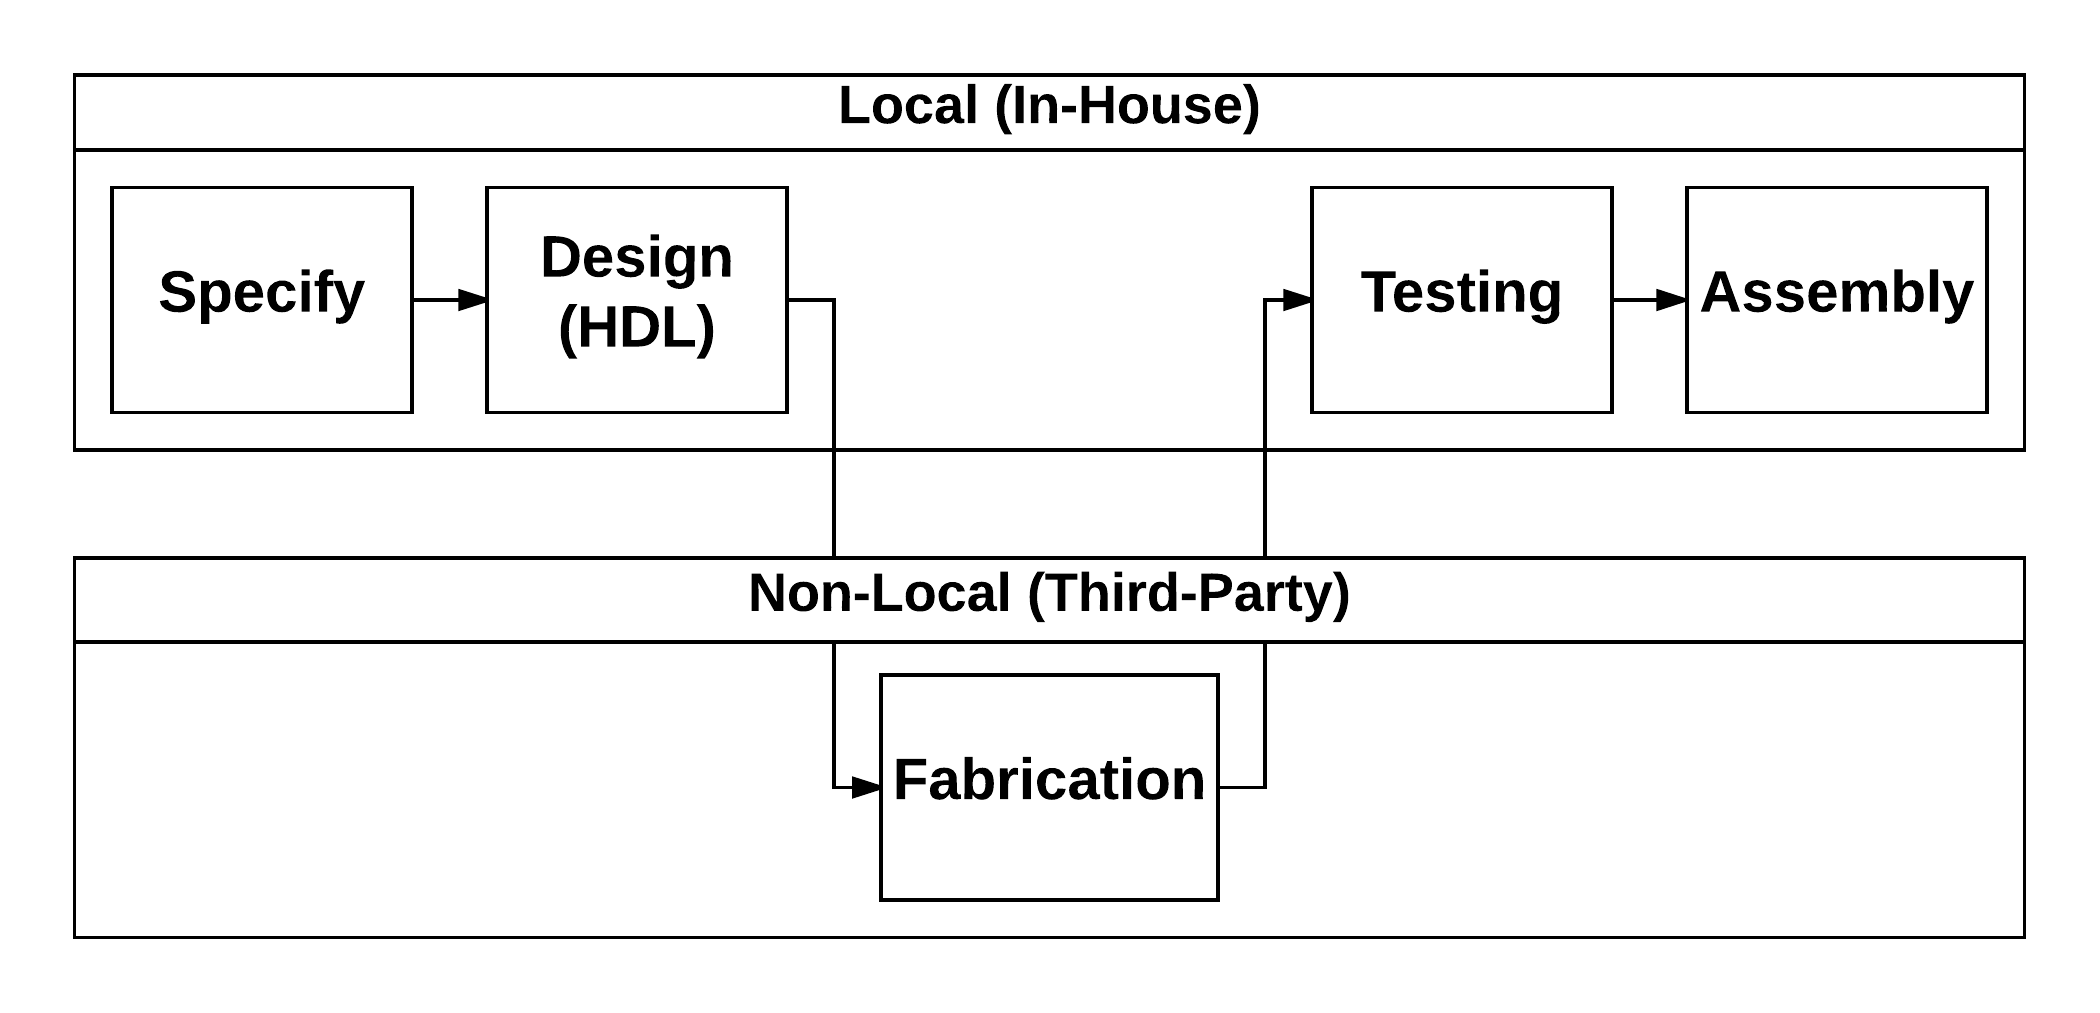
\includegraphics[width=1\linewidth]{figures/Concept}
	\caption[FPGA Life-Cycle]{FPGA Life-Cycle}
	\label{fig:Concept}
\end{figure}

Figure~\ref{fig:methodologyOverview} shows an overview of the trojan detection scheme.
\acrshort{FPGA} designs are written in a \acrfull{HDL}.
\Xilinx provides a series of \acrfull{UI} or command line tools to process the design known as the 'tool-chain'.
The tool chain generates a series of files that are used for a variety of purposes.
The Bit file is a binary representation of the design to be implemented.
It is referred to as the \gls{Bitstream} or Configuration \gls{Bitstream} and is the final form which is loaded into the device.
\begin{figure}
	\centering
	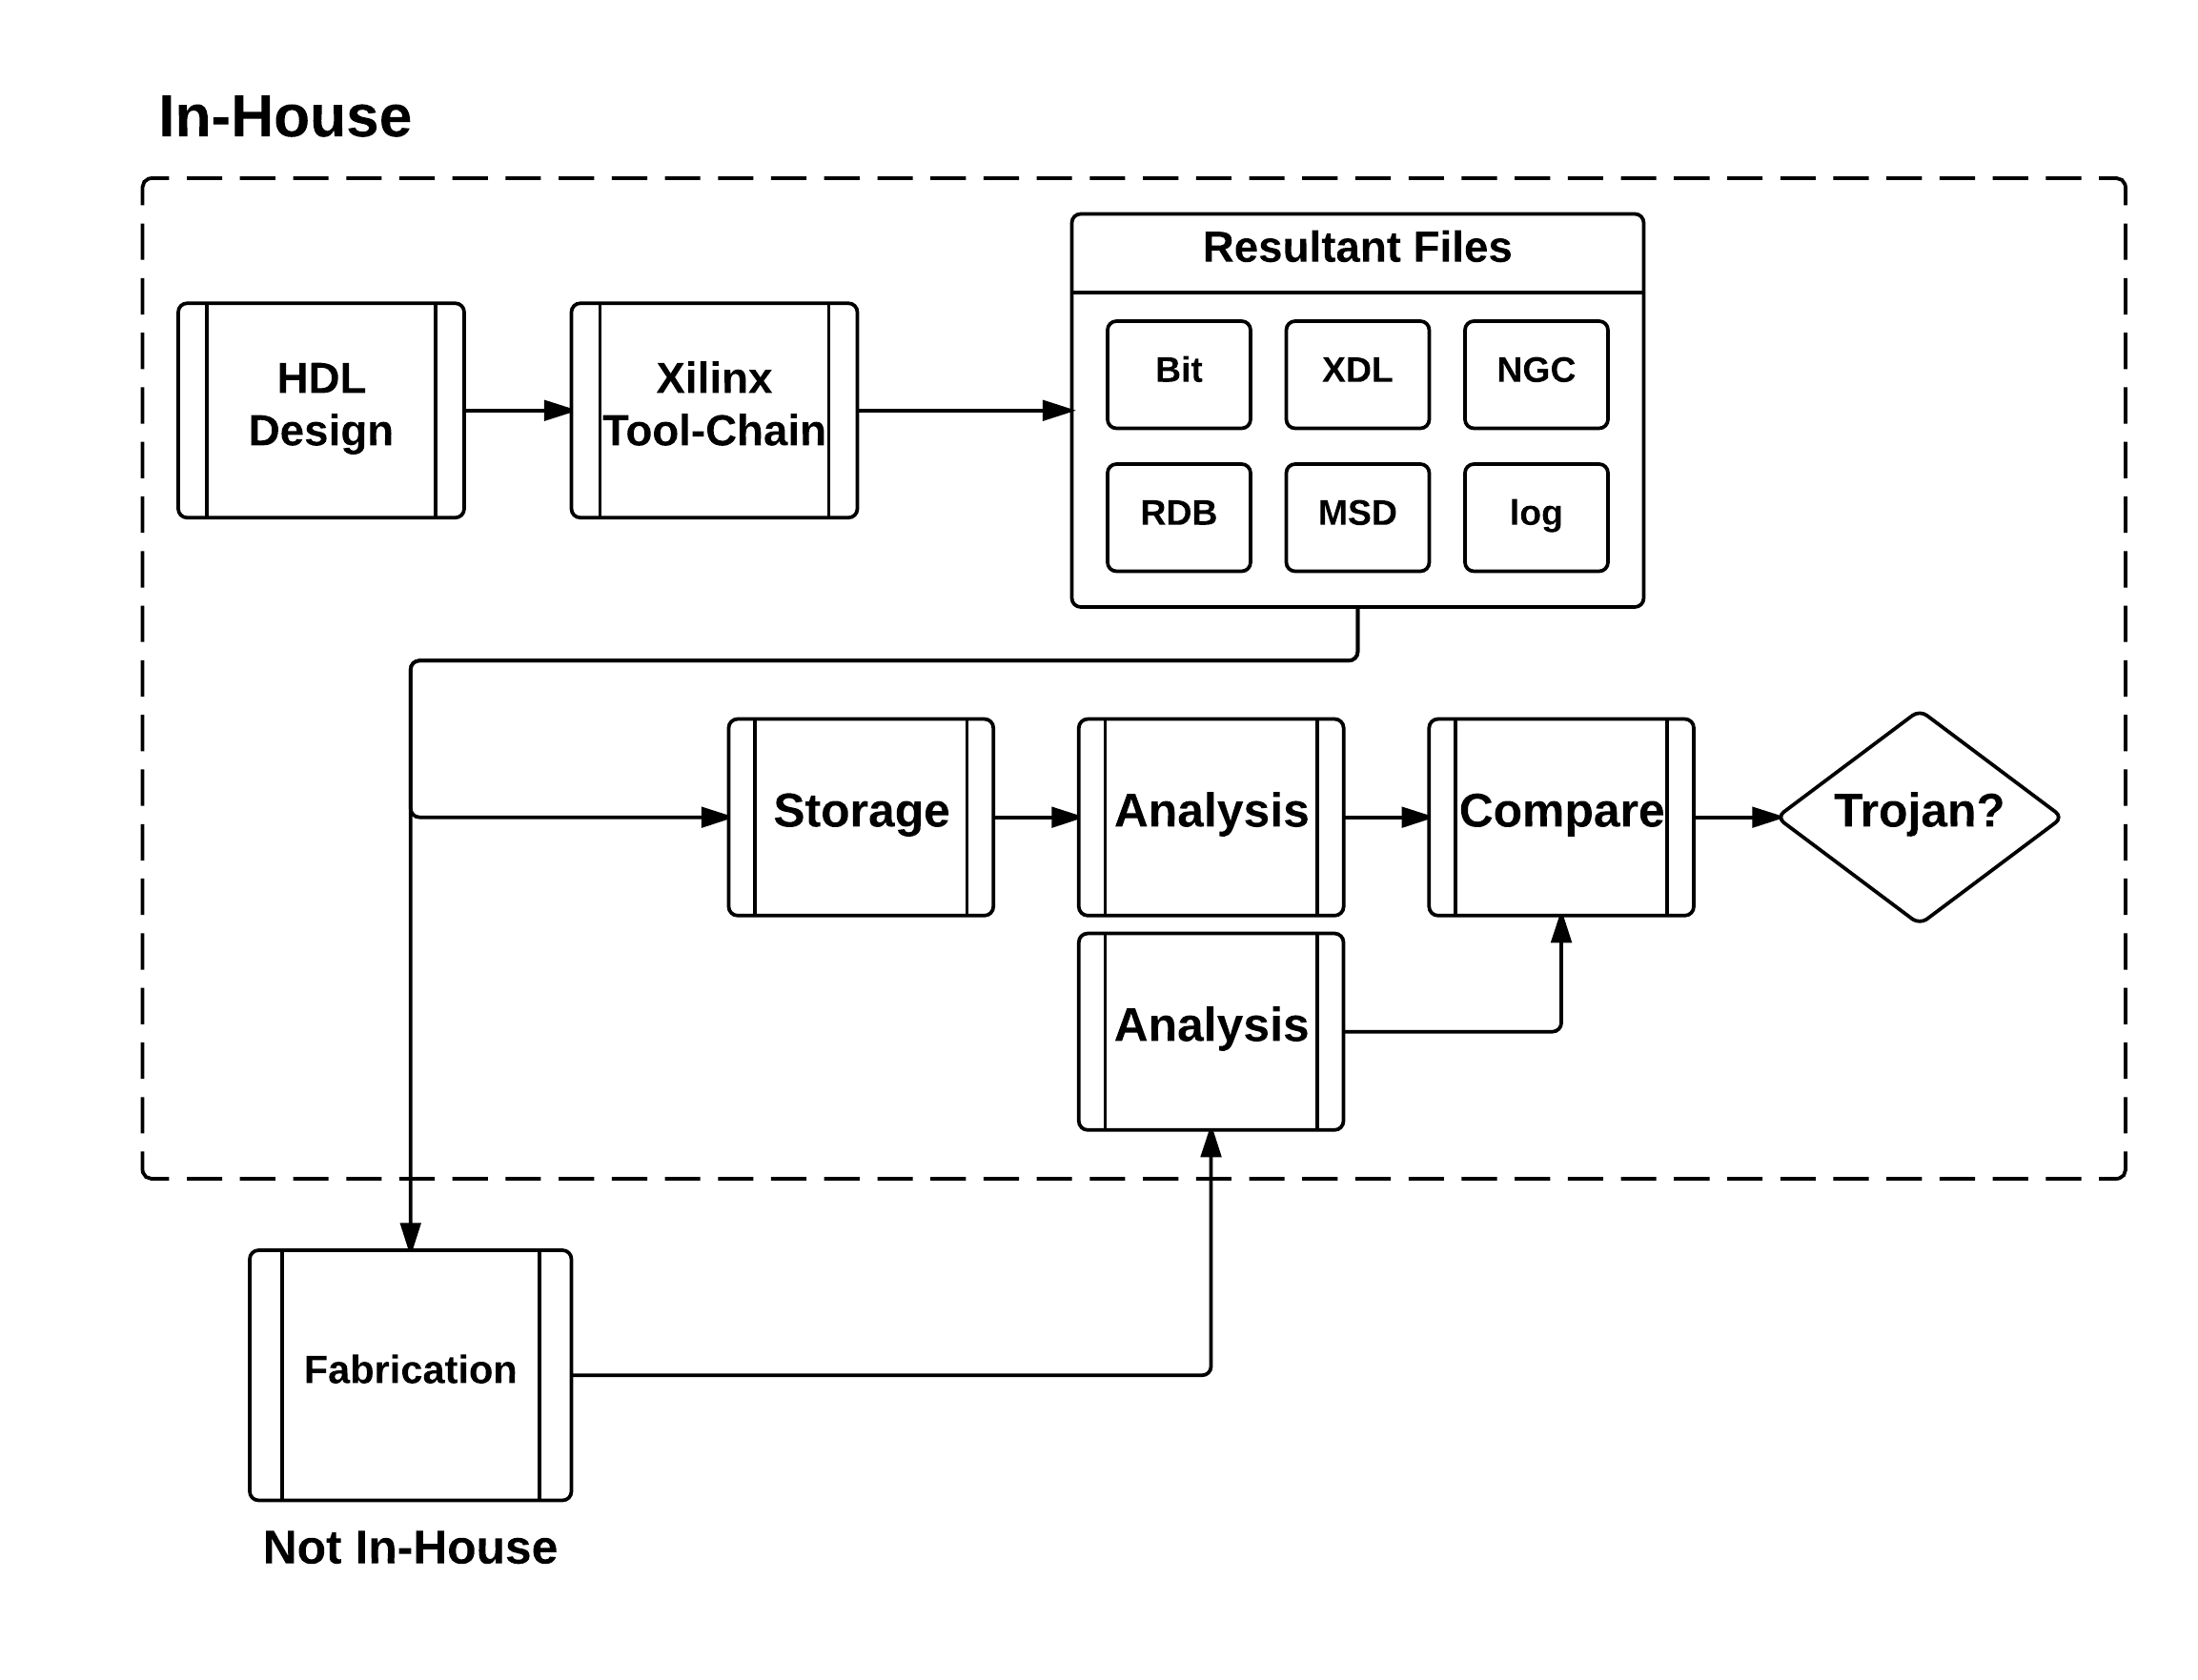
\includegraphics[width=1\linewidth]{Figures/methodologyOverview}
	\caption[Methodology Overview]{Methodology Overview}
	\label{fig:methodologyOverview}
\end{figure}
This Bit file is also one of the primary files sent to the fabrication house where it will be implemented onto the batch of devices ordered.
The resultant files are kept in secure storage while a copy is sent to be fabricated; these 'clean' copies are reffered to as \gls{golden}.
Though it is known that fabrication houses will often attempt to make optimizations on designs this methodology requires that no such efforts are made.
When the completed batch of fabricated chips are returned the \gls{Bitstream} is extracted via the method described in section~\ref{sec:bitstreamExtraction}. 
That which is extracted is referred to as the \gls{target} \gls{Bitstream}.
The \gls{golden} and \gls{target} \gls{Bitstream}s are analyzed in conjunction to detect differences, described in section~\ref{sec:frameComparison}.
Any discovered differences are then attributed to the corresponding component in the architecture, described in section~\ref{sec:tileMapping}.
Finally, descriptive attributes presented in section~\ref{sec:topology} are returned to the user, described in section~\ref{sec:trojanAttributes}. 

\section{FPGA Architecture and Configuration} \label{sec:architectureAndConfig}
A \Xilinx \acrfull{FPGA} is comprised of a matrix of blocks referred to as the 'gate-array' and is shown in Figure~\ref{fig:FPGA}.
A device can contain anywhere from a couple hundred to a few thousand blocks; they are arranged into columns by type.
A block will consist of one or multiple tiles depending on the type.
A tile is a component specific to a particular function such as \acrfull{IO}, design logic, memory...etc but their detailed functionality can be configured by the user.
An \acrshort{FPGA} may have over one-hundred different types of tiles however each column is comprised entirely by a single block type.
Columns are separated by clock regions as shown by the dashed lines in Figure~\ref{fig:FPGA}.
Each region is an independent array of blocks that uses a dedicated clock resource; this minimizes clock skew from causing undesired timing delays.
\begin{figure}[h]
	\centering
	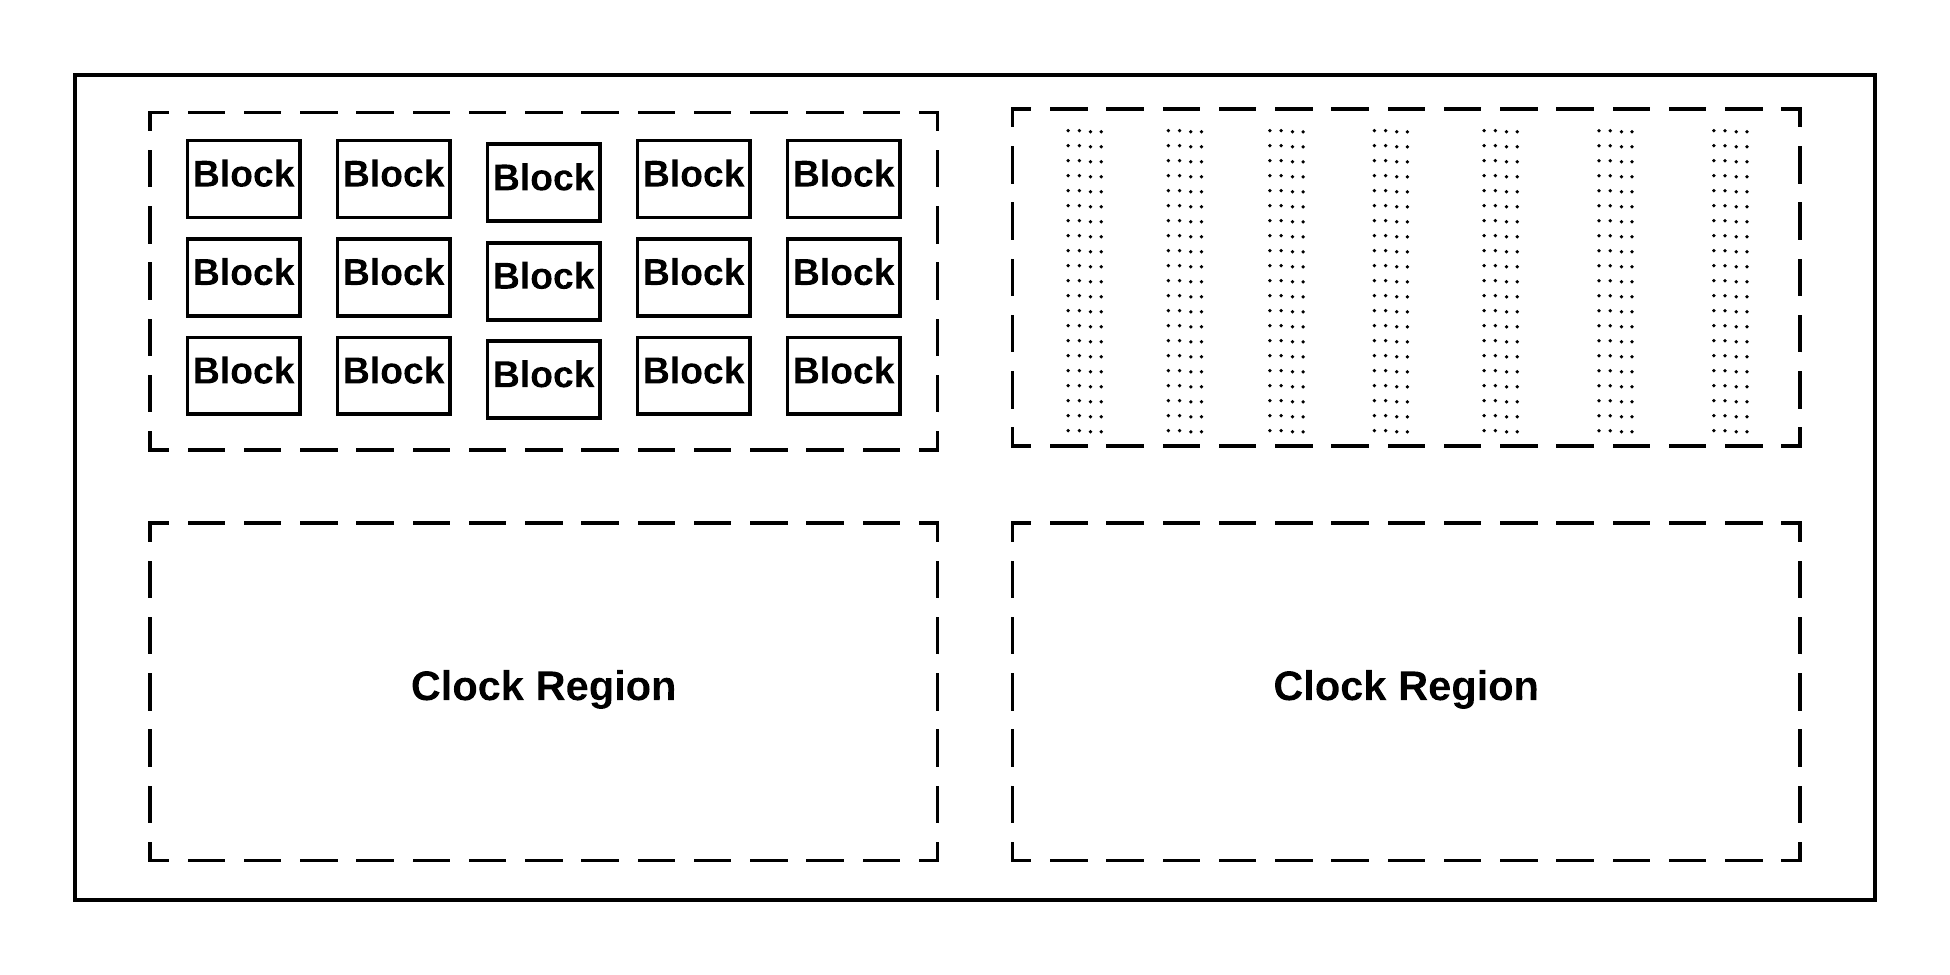
\includegraphics[width=1\linewidth]{figures/FPGA}
	\caption[Rudimentary Layout of a Virtex Gate-Array]{Rudimentary Layout of a Virtex Gate-Array}
	\label{fig:FPGA}
\end{figure}
Though each tile has a designated purposes (ex. \acrfull{IO}, \acrfull{CL}, memory...etc) their functionality can be configured by the user; this is how designs are implemented on a device.
The configuration of each tile is dictated by the \gls{Bitstream}. 
To improve performance the contents of the gate-array is referred to as dynamic.
A dynamic device is unable to retain the contents of its memory when it looses power.
To prevent having to plug in a device and download the configuration every time it is powered on, an external static memory device (i.e. retains its contents with loss of power) holds the \gls{Bitstream}. 
When an \acrshort{FPGA} is powered on the \gls{Bitstream} is loaded from the external memory (often \acrfull{SRAM}) into the gate-array, as can be seen in Figure~\ref{fig:architecture}.

\begin{figure}
\centering
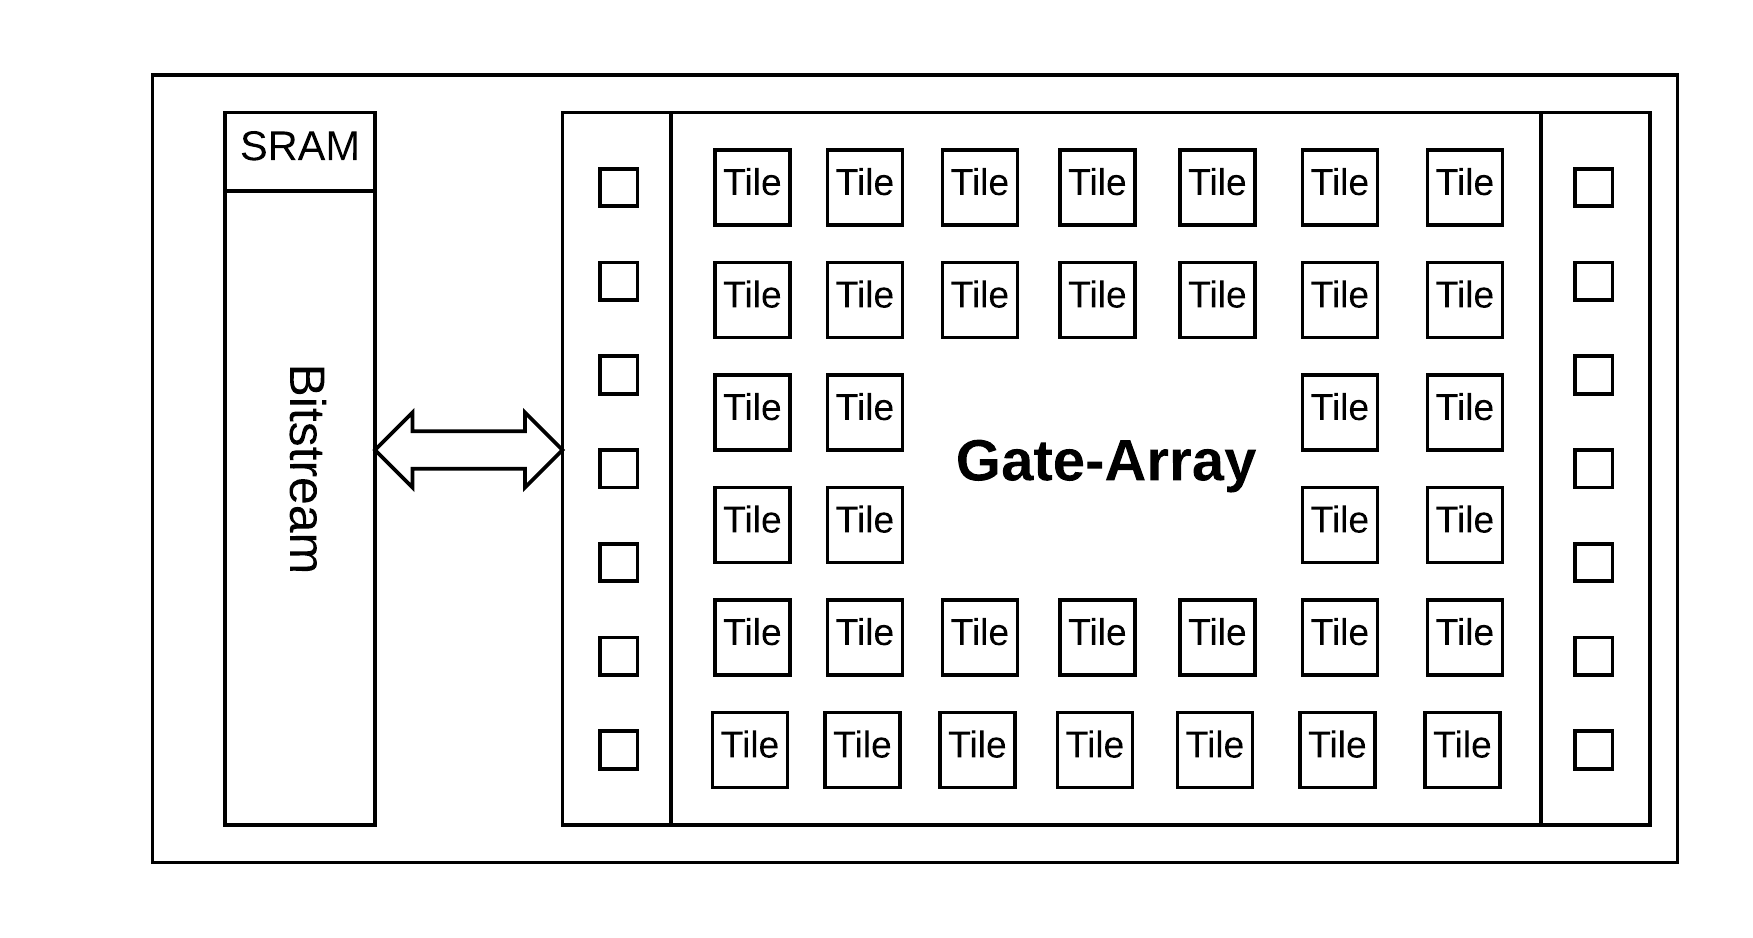
\includegraphics[width=0.9\linewidth]{Figures/architecture}
\caption[FPGA Device Layout]{FPGA Device Layout}
\label{fig:architecture}
\end{figure}

\section{The \acrshort{FPGA} Bitstream} \label{sec:fpgaBitStream}
The \Xilinx bitstream is organized into 'frames'.
A frame is a string of single bits that span from the top to the bottom of a clock region of a device as seen in the top-right quadrant of Figure~\ref{fig:FPGA}.
Frame affects every block in a column and multiple horizontally adjacent frames are required to configure an entire column.
They are uniquely identified by a 32-bit address and are the smallest addressable element.
The composition of the frame address is fairly consistent across the \Xilinx catalog however there are small differences between device families.
The following is the structure of the Virtex-5 family frame address scheme according to~\cite{virtex5ConfigGuide}.
The make-up of a frame address is shown in Table~\ref{tbl:frameAddress}.
\begin{table}[h]
	\centering
	\caption{Frame Address}
	\label{tbl:frameAddress}
	\resizebox{\textwidth}{!}{
		\begin{tabular}{|c|c|c|c|c|c|c|c|c|c|c|c|c|c|c|c|c|c|c|c|c|c|c|c|c|c|c|c|c|c|c|c|}
			\hline
			\multicolumn{8}{|c|}{Unused} & \multicolumn{3}{c|}{BA} & T & \multicolumn{5}{c|}{Row Address} & \multicolumn{8}{c|}{Major Address} & \multicolumn{7}{c|}{Minor Address} \\ \hline
			31 & 30 & 29 & 28 & 27 & 26 & 25 & 24 & 23 & 22 & 21 & 20 & 19 & 18 & 17 & 16 & 15 & 14 & 13 & 12 & 11 & 10 & 9 & 8 & 7 & 6 & 5 & 4 & 3 & 2 & 1 & 0 \\ \hline
			0 & 0 & 0 & 0 & 0 & x & x & x & x & x & x & x & x & x & x & x & x & x & x & x & x & x & x & 0 & 0 & 0 & 0 & 0 & 0 & 0 & 0 & 0 \\ \hline
		\end{tabular}		
	}
\end{table}
The \acrfull{BA} identifies the block type.
\begin{itemize}
	\item BA 0: Logic type.
	\item BA 1: \acrfull{BRAM}.
	\item BA 2: \acrshort{BRAM} Interconnect.
	\item BA 3: \acrshort{BRAM} non-configuration frame.
\end{itemize}
The logic block contains the columns which provides the primary configuration for the device (\acrshort{CLBs}, \acrshort{IOBs}... etc).
The \acrshort{BRAM} columns initialize the memory for the device while the \acrshort{BRAM} Interconnect columns configure how the logic of the design interacts with the \acrshort{BRAM}.

In the case of the Virtex-5 family each clock region is composed of twenty blocks in a column separated by a horizontal clock bus as shown in Figure~\ref{fig:RowOrder}.
\begin{figure}[h]
\centering
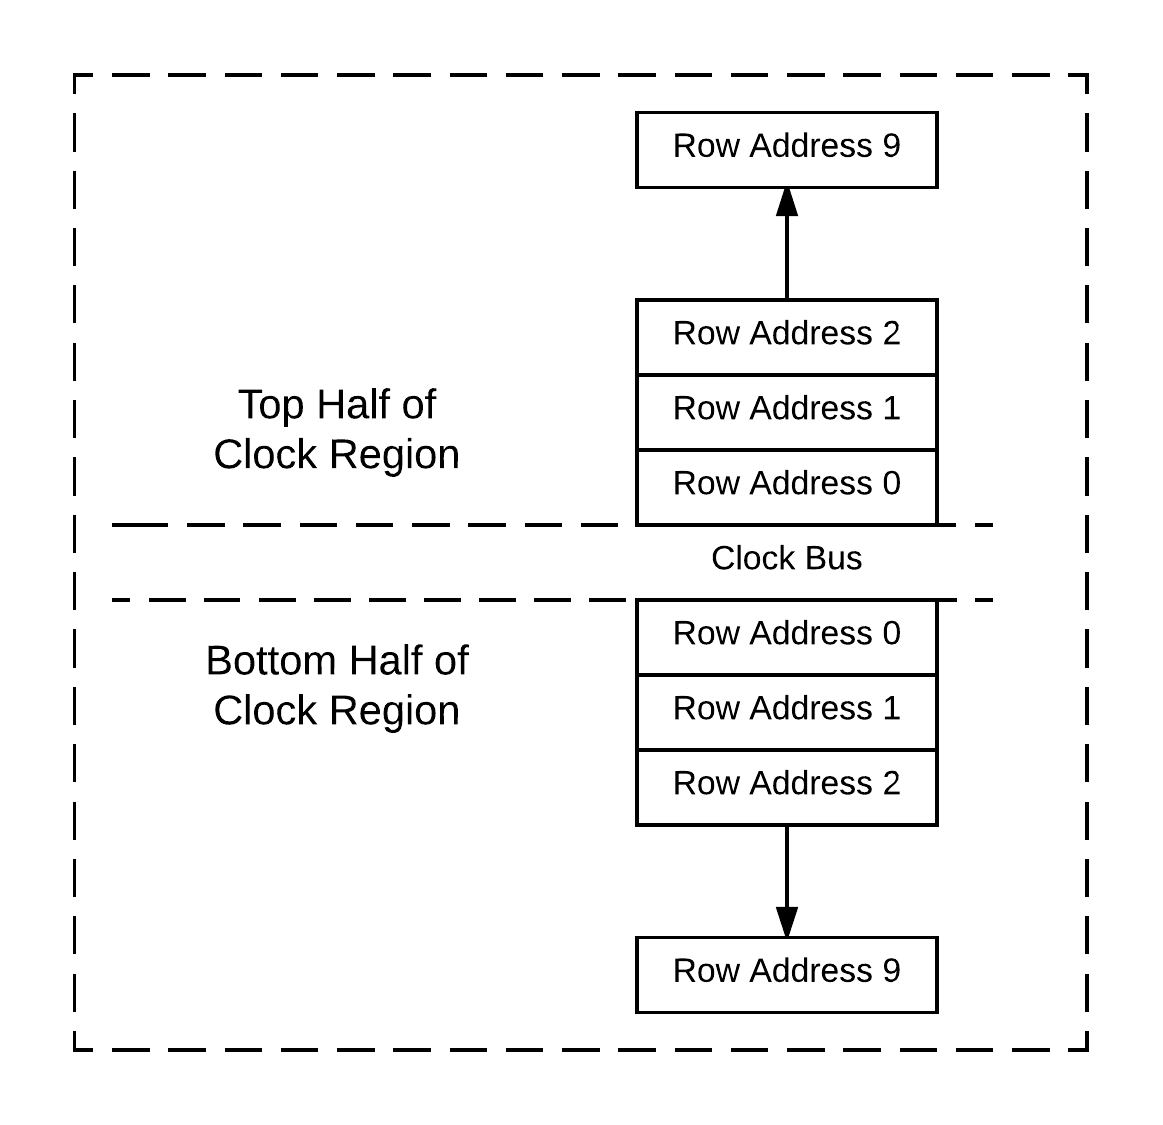
\includegraphics[width=.7\linewidth]{Figures/RowOrder}
\caption[Row Order of Virtex-5 Clock Region]{Row Order of Virtex-5 Clock Region}
\label{fig:RowOrder}
\end{figure}
Each row of blocks is given a row value in it's address that increments away from the clock bus starting at 0. 
The frame address includes a Top indicator bit in position 20 that indicates whether the specified row is above or below the horizontal clock bus.
The major address specifies the block within the row.
These addresses are numbered from left to right and begin at 0.
The minor address indicates the frame number within a column. 
Table~\ref{tbl:minorAddressNumbers} provides the number of frames per column type.
\begin{table}[]
	\centering
	\caption{Number of Frames (minor addresses) per Column}
	\label{tbl:minorAddressNumbers}
	\begin{tabular}{|c|c|}
		\hline
		Block             & Number Of Frames \\ \hline
		CLB               & 36               \\ \hline
		DSP               & 28               \\ \hline
		\acrshort{BRAM} & 30               \\ \hline
		IOB               & 54               \\ \hline
		Clock             & 4                \\ \hline
	\end{tabular}
\end{table}
The number of frames given in Table~\ref{tbl:minorAddressNumbers} corresponds to the block in the column.
As described in section~\ref{sec:architectureAndConfig} a block may contain multiple tiles.
In a CLB column a block consists of an interconnect column and a \acrshort{CLB}.
To further understand how frames configure tiles a mapping must be made between each frame and the corresponding tile.
This is described in section~\ref{sec:tileMapping}.
%The logic block type has sub block-type columns:
%\begin{itemize}
%	\item \acrfull{CLB} columns which configure the logic blocks, routing and the majority of the interconnect.
%	\item \acrfull{IOB} columns which configure the I/O voltage standard.
%	\item \acrfull{IOI} columns which configure the \acrshort{IOB} registers, multiplexers and buffers.
%	\item \acrfull{GCLK} columns global clock resources including clock buffers and the \acrfull{DCM}.
%\end{itemize}
 
\section{\gls{Bitstream} Extraction} \label{sec:bitstreamExtraction}
In order to detect any trojans in the \gls{target} device the configuration \gls{Bitstream} will need to be recovered.
As mentioned in section~\ref{sec:architectureAndConfig} the \gls{Bitstream} is stored in a memory unit external to the gate-array.
All \Xilinx devices provide a feature known as \gls{Readback}.
There are two styles of \gls{Readback}; \gls{Readback} verify and \gls{Readback} Capture.
The \gls{Readback} capture method provides a large quantity of debug information which is not needed; \gls{Readback} verify will be used.
\gls{Readback} verify is the process where the device is put into a 'frozen' state during run-time and all of the configuration bits are returned from the gate-array to the \acrshort{SRAM}. 
The results can then be uploaded to a \acrfull{PC} for analysis.
This process overwrites the original frame data in the \acrshort{SRAM} with the values which actually configured the device. 
By using this method rather than simply reading the \acrshort{SRAM} it ensures that what is tested in section~\ref{sec:frameComparison} is actually what configured the device.
This minimizes risk of tampered external memory units or configuration mechanics. 
\section{Frame Comparison} \label{sec:frameComparison}
\section{Tile Mapping} \label{sec:tileMapping}
\section{Trojan Attributes} \label{sec:trojanAttributes}



%This is where you go all out and tell us all about your new discovery and research related to the problem in the previous chapter. No arrogant sweeping statements which cannot be fully justified, but no false modesty either. You must impress your reader that you have accomplished something.
%
%Simply summarized, this chapter should be comprised of at least two main sections, each with appropriate subsections. The first section should describe:
%\begin{itemize}
%\item {what the new approach is;}
%\item {what is really totally new;}
%\item {what is incrementally new;}
%\item {what you built upon.}
%\end{itemize}
%
%The second part should describe fully how the new approach works, both with the overall theoretical exposition (e.g. an algorithm) and with as many examples as necessary for clarity. Remember that if the reader does not understand fully, you will get a lot of questions and doubts. Good examples, good figures, good diagrams with super clear tutorial explanations can be a joy to read and make even a small contribution appear to be more impressive. Are you afraid that if you are too tutorial your work will not seem as deep and difficult? Only shallow people will make such a superficial evaluation, have trust instead in the wisdom of your supervisory committee.
%
%Use at least one good example throughout, and even better if this is one of the examples you used in Chapter 2 to describe the original problem.
%
%By the way, this would be the first chapter I would write. This is what I know best right now, as I just finished working on it. It is clear to me and on the tip of my fingers. Start with your strengths! The second chapter I would write is the next one about the experiments, followed closely by chapter 2 describing the problem. It may not seem intuitive to you, but it works and it is the most productive way I ever found to finish a document.
%
%
%\input chapters/3/sec_latexhelp

	\startchapter{Software Implementation}
\label{chapter:implementation}

\section{Technologies Used}
\section{Design}
\section{\acrfull{UI}}
	\startchapter{Evaluation, Analysis and Comparisons}
\label{chapter:eval}

For a Master's research this chapter represents the critical part where \textbf{you} are truly evaluated to determine whether you should be given your degree. Even more so for a PhD. Consider carefully what the University calendar states regarding the expectations for a master's thesis, paraphrased here.

\begin{enumerate}
\item {\textit{A Master�s thesis is an original lengthy essay.} The main implication here is that the essay is original, that is, it is completely newly written by you and does not contain any writings from others unless precisely quoted. Any paraphrased items must be cited.}
\item {\textit{It must demonstrate that:}
    \begin{itemize}
    \item {students understand research methods;}
    \item {students are capable to employ research methods;}
    \item {students demonstrate command of the subject.}
    \end{itemize}}
\item {\textit{The work may be based on:}
    \begin{itemize}
    \item {original data;}
    \item {original exercise from scholarly literature;}
    \item {data by others.}
    \end{itemize}}
\item {\textit{The work must show that:}
    \begin{itemize}
    \item {appropriate research methods have been used;}
    \item {appropriate methods of critical analysis supplied.}
    \end{itemize}}
\item {\textit{The work must contain:}
    \begin{itemize}
    \item {evidence of some new contribution;}
    \item {evidence of a new perspective on existing knowledge.}
    \end{itemize}}
\end{enumerate}

Only the last point uses the attribute \textit{new} and it refers almost entirely to giving a new perspective and analysis, even if based on data from others. This truly implies that this current chapter on evaluation and analysis of results is the most important and must be written with care. You are demonstrating here that, even if given data and methods from others, your skills of critical judgment and analysis are now at the level that you can give professional evaluations.

Things are slightly different for a PhD. According to the Graduate Calendar: \\ 
\textit{a doctoral dissertation must embody original work and constitute a significant contribution to knowledge in the candidate's field of study. It should contain evidence of broad knowledge of the relevant literature, and should demonstrate a critical understanding of the works of scholars closely related to the subject of the dissertation. Material embodied in the dissertation should, in the opinion of scholars in the field, merit publication.}

\textit{The general form and style of dissertations may differ from department to department, but all dissertations shall be presented in a form which constitutes an integrated submission. The dissertation may include materials already published by the candidate, whether alone or in conjunction with others. Previously published materials must be integrated into the dissertation while at the same time distinguishing the student's own work from the work of other researchers. At the final oral examination, the doctoral candidate is responsible for the entire content of the dissertation. This includes those portions of co-authored papers which comprise part of the dissertation.}

The second paragraph makes it clear that one must emphasize what is new and different from others, without arrogance, yet without being too subtle either. The first paragraph implies that for a PhD it is required that one approached an important open problem and gave a new solution altogether, making chapters 3, 4, 5 all part of the body of research being evaluated. In fact at times even the problem may be entirely new, thus including chapter 2 in the examination. This is in contrast to a Master's degree where the minimum requirement is for chapter 5 to be original.




	\startchapter{Contributions}
\label{chapter:contributions}


	\appendix
	\startappendix{Software Implementations}
\label{chapter:appendix}

\section{Technologies Used}
\subsection{\Xilinx}
\Xilinx is one of the two largest manufacturers of \acrshort{FPGA}s; their devices are considerably more popular than their competitors.
The configuration of devices employs a well known series of steps referred to as the \Xilinx 'tool-chain'~\cite{xilnxDevManual}.
The 'tool-chain' not only compiles user designs and constraints into the configuration \gls{Bitstream} but performs a series of complex operations to optimize designs and effectively implement them on any \Xilinx model of the user's choosing.
\begin{enumerate}
	\item \textbf{\gls{sch2hdl}}: \glsdesc{sch2hdl}
	\item \textbf{\gls{XST}}: \glsdesc{XST}
	\item \textbf{\gls{MAP}}: \glsdesc{MAP}
	\item \textbf{\gls{PAR}}: \glsdesc{PAR}
	\item \textbf{\gls{ngdbuild}}: \glsdesc{ngdbuild}
	\item \textbf{\gls{trce}}: \glsdesc{trce}
	\item \textbf{\gls{Bitgen}}: \glsdesc{Bitgen}
\end{enumerate}
Each step produces a series of files that are used for a variety of purposes. 
Often the resultant files are used by the subsequent step but some are intended for user information.
The \gls{ngdbuild} tool generates what is known as the netlist for the design.
The netlist is a description of the connectivity of the circuit implemented on the device. 
The generated netlist is in a non human-readable format in an 'ndc' file.
Fortunately, \Xilinx provides an additional tool called \gls{xdl2ndc} which allows the conversion to the human-readable \acrfull{XDL}.
\subsubsection{\acrfull{XDL}} \label{sec:XDL}
The \acrfull{XDL} is a human-readable ASCII format; though it is not actively part of the 'tool-chain' it is considered a native netlist format for describing and representing \acrshort{FPGA} designs~\cite{xdlTutorial}. 
In a netlist, a 'part' is a human-defined component which is to be implemented.
Netlists either contain or refer to descriptions of the parts used and where in the device they are implemented.
When a part is used it is called an 'instance'; thus each 'instance' has a definition, sometimes referred to as a master.

An \acrshort{XDL} file contains two sections, the instance placement and configuration section, and the net routing section. 
The placement and configuration section provides a list of every instance in a design. 
Their descriptions include all of the configuration details required for their implementation on a component (power settings, logic, timing configurations... etc).
In the \Xilinx jargon, a net refers to any electrical path between two components; more specifically, a net describes a communication channel.
The gate-array of a \Xilinx device is composed of a grid of wires.
These wires can be fused together by \acrfull{PIP} to make a useful connection between two components, thus creating a net.
The output-pin of a net receives the signal from the transmitting component while the input-pin delivers the signal to the corresponding receiver.
The \acrshort{PIP}s in-between the end-points dictate the path the signal takes between the two components.
The net routing section of the \acrshort{XDL} file describes every path in the design.
Combined, these two sections completely describe a design and how it is implemented.
The information provided by the \acrshort{XDL} file is used by the \NameNoPeriod to relate any of the effects of a discovered trojan to the user's intended operation. 
\subsubsection{XDLRC} \label{sec:XDLRC}
The \acrshort{XDL} file describes the design implemented on a device.
From this a lot of information regarding the composition of a \Xilinx device can be learned but it does not provide the entire description; only what has been used by the design.
The \gls{xdl2ndc} command line tool provides an option to generate a resource report file referred to as an XDLRC file. 
A XDLRC file describes the entire architecture of a \Xilinx \acrshort{FPGA}.

\ConditionSize
\begin{lstlisting}[label={lst:xdlrc}, language=Python, caption={A hierarchical XDLRC resource description of a Spartan 6 FPGA consisting of a header, a tile section, and a trailing device summary~\cite{xdlTutorial}}]
#Header section
(xdl_resource_report v0.2 xc6slx16csg324-3 spartan6
# Device Level Dimensions
(tiles 73 62
...
#Configurable logic block with two slices
(tile 4 6 CLEXL_X1Y61 CLEXL 2
(primitive_site SLICE_X0Y61 SLICEL internal 45
(pinwire A1 input L_A1)
...
(primitive_site SLICE_X1Y61 SLICEX internal 43
...
(pinwire D output XX_D)
...)
# Interconnect tile
(tile 4 5 INT_X1Y61 INT 1
...
(wire EE2B0 2
(conn CLEXM_X2Y61 CLEXM_EE2M0)
(conn INT_BRAM_X3Y61 EE2E0)
...
# Programmable Interconnect Points
(pip INT_X1Y61 EE2E0 -> EE2B0)
(pip INT_X1Y61 EE4E0 -> EE2B0)
(pip INT_X1Y61 EL1E_S0 -> LOGICIN_B9)
...)
# summary
(summary tiles=4526 sites=5378 sitedefs=46 numpins=157962 numpips=5782505))
\end{lstlisting}
\normalsize

Listing~\ref{lst:xdlrc} provides an example of the XDLRC format.
The report begins with a header describing the device.
It then reports that the overall architecture contains a matrix of tiles, 73-wide and 62-tall.
Further down is a configurable logic block at coordinate (4,6) and an interconnect tile at coordinate (4,5).
Each of these tile descriptions provide details of the subcomponents they contain, pinwires, \acrshort{PIP}s, slices...etc.
The \gls{xdl2ndc} tool is capable of generating a variety of different XDLRC files for a device, ranging in the level of detail.
The smaller files can be around 10MB while the fully detailed descriptions can reach 7GB in size.
\subsection{Java} \label{sec:java}
Java is a powerful and general-purpose programming language. 
It is specifically designed to be as independent as possible.
The original developer, James Gosling, intended the language to allow developers a comfortable implementation experience with seamless deployment. 
The custodians of the Java language, Sun Microsystems, promote the slogan 'write-once, run anywhere'.  
\NameNoPeriod was written in Java primarily in order to interface with the \acrshort{API} known as \RapidSmith which is described in section~\ref{sec:rapidSmith}.
However, Java additionally allows the \NameNoPeriod to be a compact, cross-platform application.
The Java language provides a native \acrfull{GUI} toolkit known as \SwingEnd.
\Swing is an \acrshort{API} that is part of Oracle's Java Foundation Classes; in other words it is readily available to all users of Java.
It provides a simple to use programming structure for creating sophisticated \acrshort{UIs}.
The \NameNoPeriod employs Java and Java \Swing.
This implies that the only requirement for a user to take advantage of the power of the \NameNoPeriod is to have Java installed; which most modern machines do.

\subsection{\RapidSmith} \label{sec:rapidSmith}
\RapidSmith is an \acrfull{APIs} written in Java that enables \acrfull{CAD} tool creation for \Xilinx \acrshort{FPGA}s~\cite{rapidSmith}.
Its purpose is to be used as a rapid prototyping platform for experimentation and research.
The code is free to use and readily accessible.
It was chosen as a supporting library for the \NameNoPeriod for several reasons.
First, the code base provides a series of class structures that astutely mirror the architecture of \Xilinx devices.
Secondly, it provides ready-made tools for extracting the configuration frames from \gls{Bitstream} files. 
\gls{Bitstream} files are long binary sequences, without the tools provided by \RapidSmith the analysis of these files becomes an arduous task.
Finally, and most importantly, the creators of \RapidSmith have developed a means of condensing XDLRC files into a greatly compressed format referred to as a 'database' file.
The \NameNoPeriod requires considerable detail of an \acrshort{FPGA}'s architecture in order to accurately described the effects a trojan has on a design.
As mentioned in section~\ref{sec:XDLRC}, the fully detailed XDLRC files can reach 7GB in size.
Working with text-based files of this size detriments performance to an unacceptable level.
The makers of \RapidSmith have developed a compression scheme which converts the XDLRC files into a non human-readable format.
This scheme reduces the size of the XDLRC files from 7GB to 1.3MB. 
The \acrshort{API} provides the necessary interface classes for querying the compressed files.
With these compressed fies, \RapidSmith gives the \NameNoPeriod the ability to analyze the effect any discovered trojan has on a device.
\subsubsection{Class Structure} \label{sec:classStructure}
Building off of the information provided by the XDLRC architecture files, \RapidSmith provides a class structure that enables developers an easy to use interface for working with \acrshort{FPGA}s.
As described in section~\ref{sec:architectureAndConfig}, the gate-array of an \acrshort{FPGA} is composed of blocks made up of tiles.
These tiles are further composed of sub-components collectively referred to as 'primitives'.
Figure~\ref{fig:classStructures} shows the top-down construction of the \RapidSmith class structure.
The \NameNoPeriod employs both the 'Device' and 'Design' classes shown in Figures~\ref{fig:rapidSmithDevice} and~\ref{fig:rapidSmithDesign} respectively.
The \gls{Bitstream} for the \gls{golden} and \gls{target} devices are read into memory. 
A utility class which parses the \gls{Bitstream} into its configuration frames determines the model of the devices used.
The 'Device' class is configured to the correct model and then is loaded with the architecture details from the compressed XDLRC file.
The complete description of the architecture is read and loaded; every tile, primitive, wire, and how they all interconnect is stored in memory.
The \gls{golden} \acrshort{XDL} file is then loaded.
The \acrshort{XDL} file is read and the 'Design' class is similarly loaded with the user-defined design.
\begin{figure*}[h]
	\centering
	\begin{subfigure}[t]{0.5\textwidth}
		\centering
		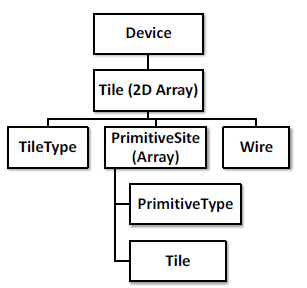
\includegraphics[height=2in]{Figures/rapidSmithDevice}
		\caption{The Device Class-Structure}
		\label{fig:rapidSmithDevice}
	\end{subfigure}%
	~ 
	\begin{subfigure}[t]{0.5\textwidth}
		\centering
		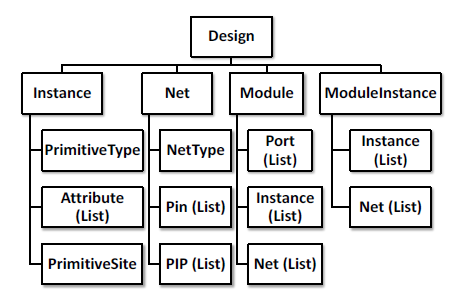
\includegraphics[height=2in]{Figures/rapidSmithDesign}
		\caption{The Design Class-Structure}
		\label{fig:rapidSmithDesign}
	\end{subfigure}
	\caption{The \RapidSmith Class Hierarchy~\cite{rapidSmithManual}}
	\label{fig:classStructures}
\end{figure*}
Not shown in Figure~\ref{fig:classStructures} are a series of utility classes.
The \gls{Bitstream} parser class reads and interprets the \gls{Bitstream} files. 
It uses a 'Frame' class to organize the \gls{Bitstream} file into an array of objects that adhere to the configuration pattern described in section~\ref{sec:architectureAndConfig}.
The frame objects are populated with the frame's 32-bit address, an array of 32-bit words which make up the frame and a series of helper methods.
\section{\Name}
\subsection{\acrfull{UI}}
Java and Java \Swing provide an easy to use \acrlong{UI} development system which produces light-weight, portable and cross platform applications.
The \NameNoPeriod employs \Swing to provide a very simplistic and easy to use interface which can be seen in Figure~\ref{fig:UI}.
To perform an analysis the user must use the \acrshort{UI} to navigate to and select the \gls{golden} \gls{Bitstream}, the \gls{target} \gls{Bitstream} and the \gls{golden} \acrshort{XDL} file via the three browse buttons on the left.
Once loaded the detection process can be launched via the 'Analyze' button.
On the right the user is able to review information specific to the trojan, which will be described in section~\ref{sec:operation}.
\begin{figure}
	\centering
	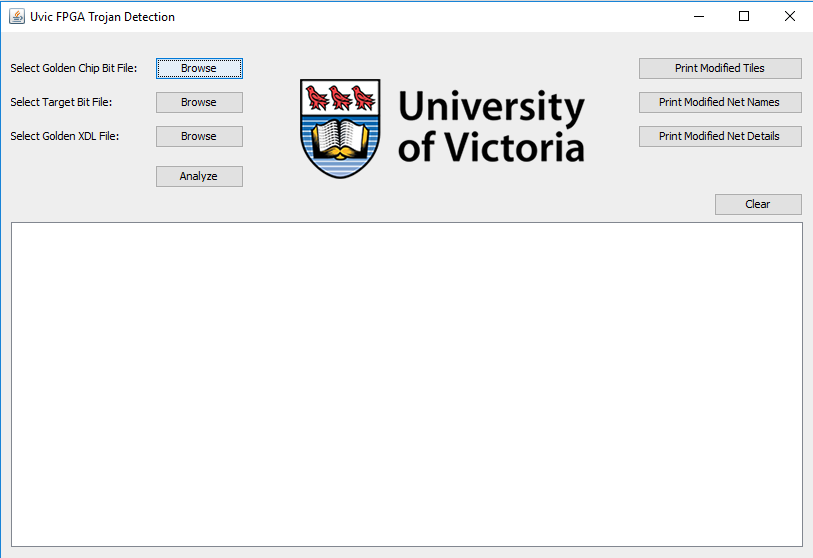
\includegraphics[width=0.96\linewidth]{Figures/UI}
	\caption[The User-Interface of the \NameNoPeriod]{The User-Interface of the \NameNoPeriod}
	\label{fig:UI}
\end{figure}

If a modification is discovered, the \NameNoPeriod analyzes it and reports a list of attributes from the taxonomy of Chapter~\ref{chapter:hardwareTrojans} which describe it.
Results are printed textually in the text window.
The attribute id-number, name, category and a brief description of the attribute are provided.
After the analysis the user is able to use the 'Print Modified Tiles' feature.
Any tile in the architecture which corresponds to a modified tile is printed to the text window. 
This provides the user with the exact location on the their device where modification took place.
The 'Print Modified Instances' feature corresponds each modified tile to the design-instance it belongs to.
\Xilinx provides schematic design views which correspond instance names to the user's design.
This can be used by the user to refer back to their design and view the trojan's effects from a high abstraction perspective.
The 'Print Modified Net Names' provides only the names of each channel that has been modified. 
Again this allows the user to relate modifications to their design.
The 'Print Modified Net Details' button provides both the names of modified nets and their corresponding list of primitives.
Finally, the 'Clear' button is a manual method of removing the text from the text-window.
\subsection{Operation} \label{sec:operation}
Figure~\ref{fig:Operation} gives a visual representation of the operating procedure of the \Name.
To perform analysis the user must submit the \gls{golden} and \gls{target} \gls{Bitstream} files.
As seen on the left of Figure~\ref{fig:Operation}, these large binary files are parsed by a utility class provided by \RapidSmith. 
The parsing utility is able to detect the model of the device by scanning the 'header' information in the files.
Different \Xilinx models use different configuration patterns.
The \gls{Bitstream} of different models may differ in a variety of features including frame size, ordering, address structure and more.
\begin{figure}[h]
	\centering
	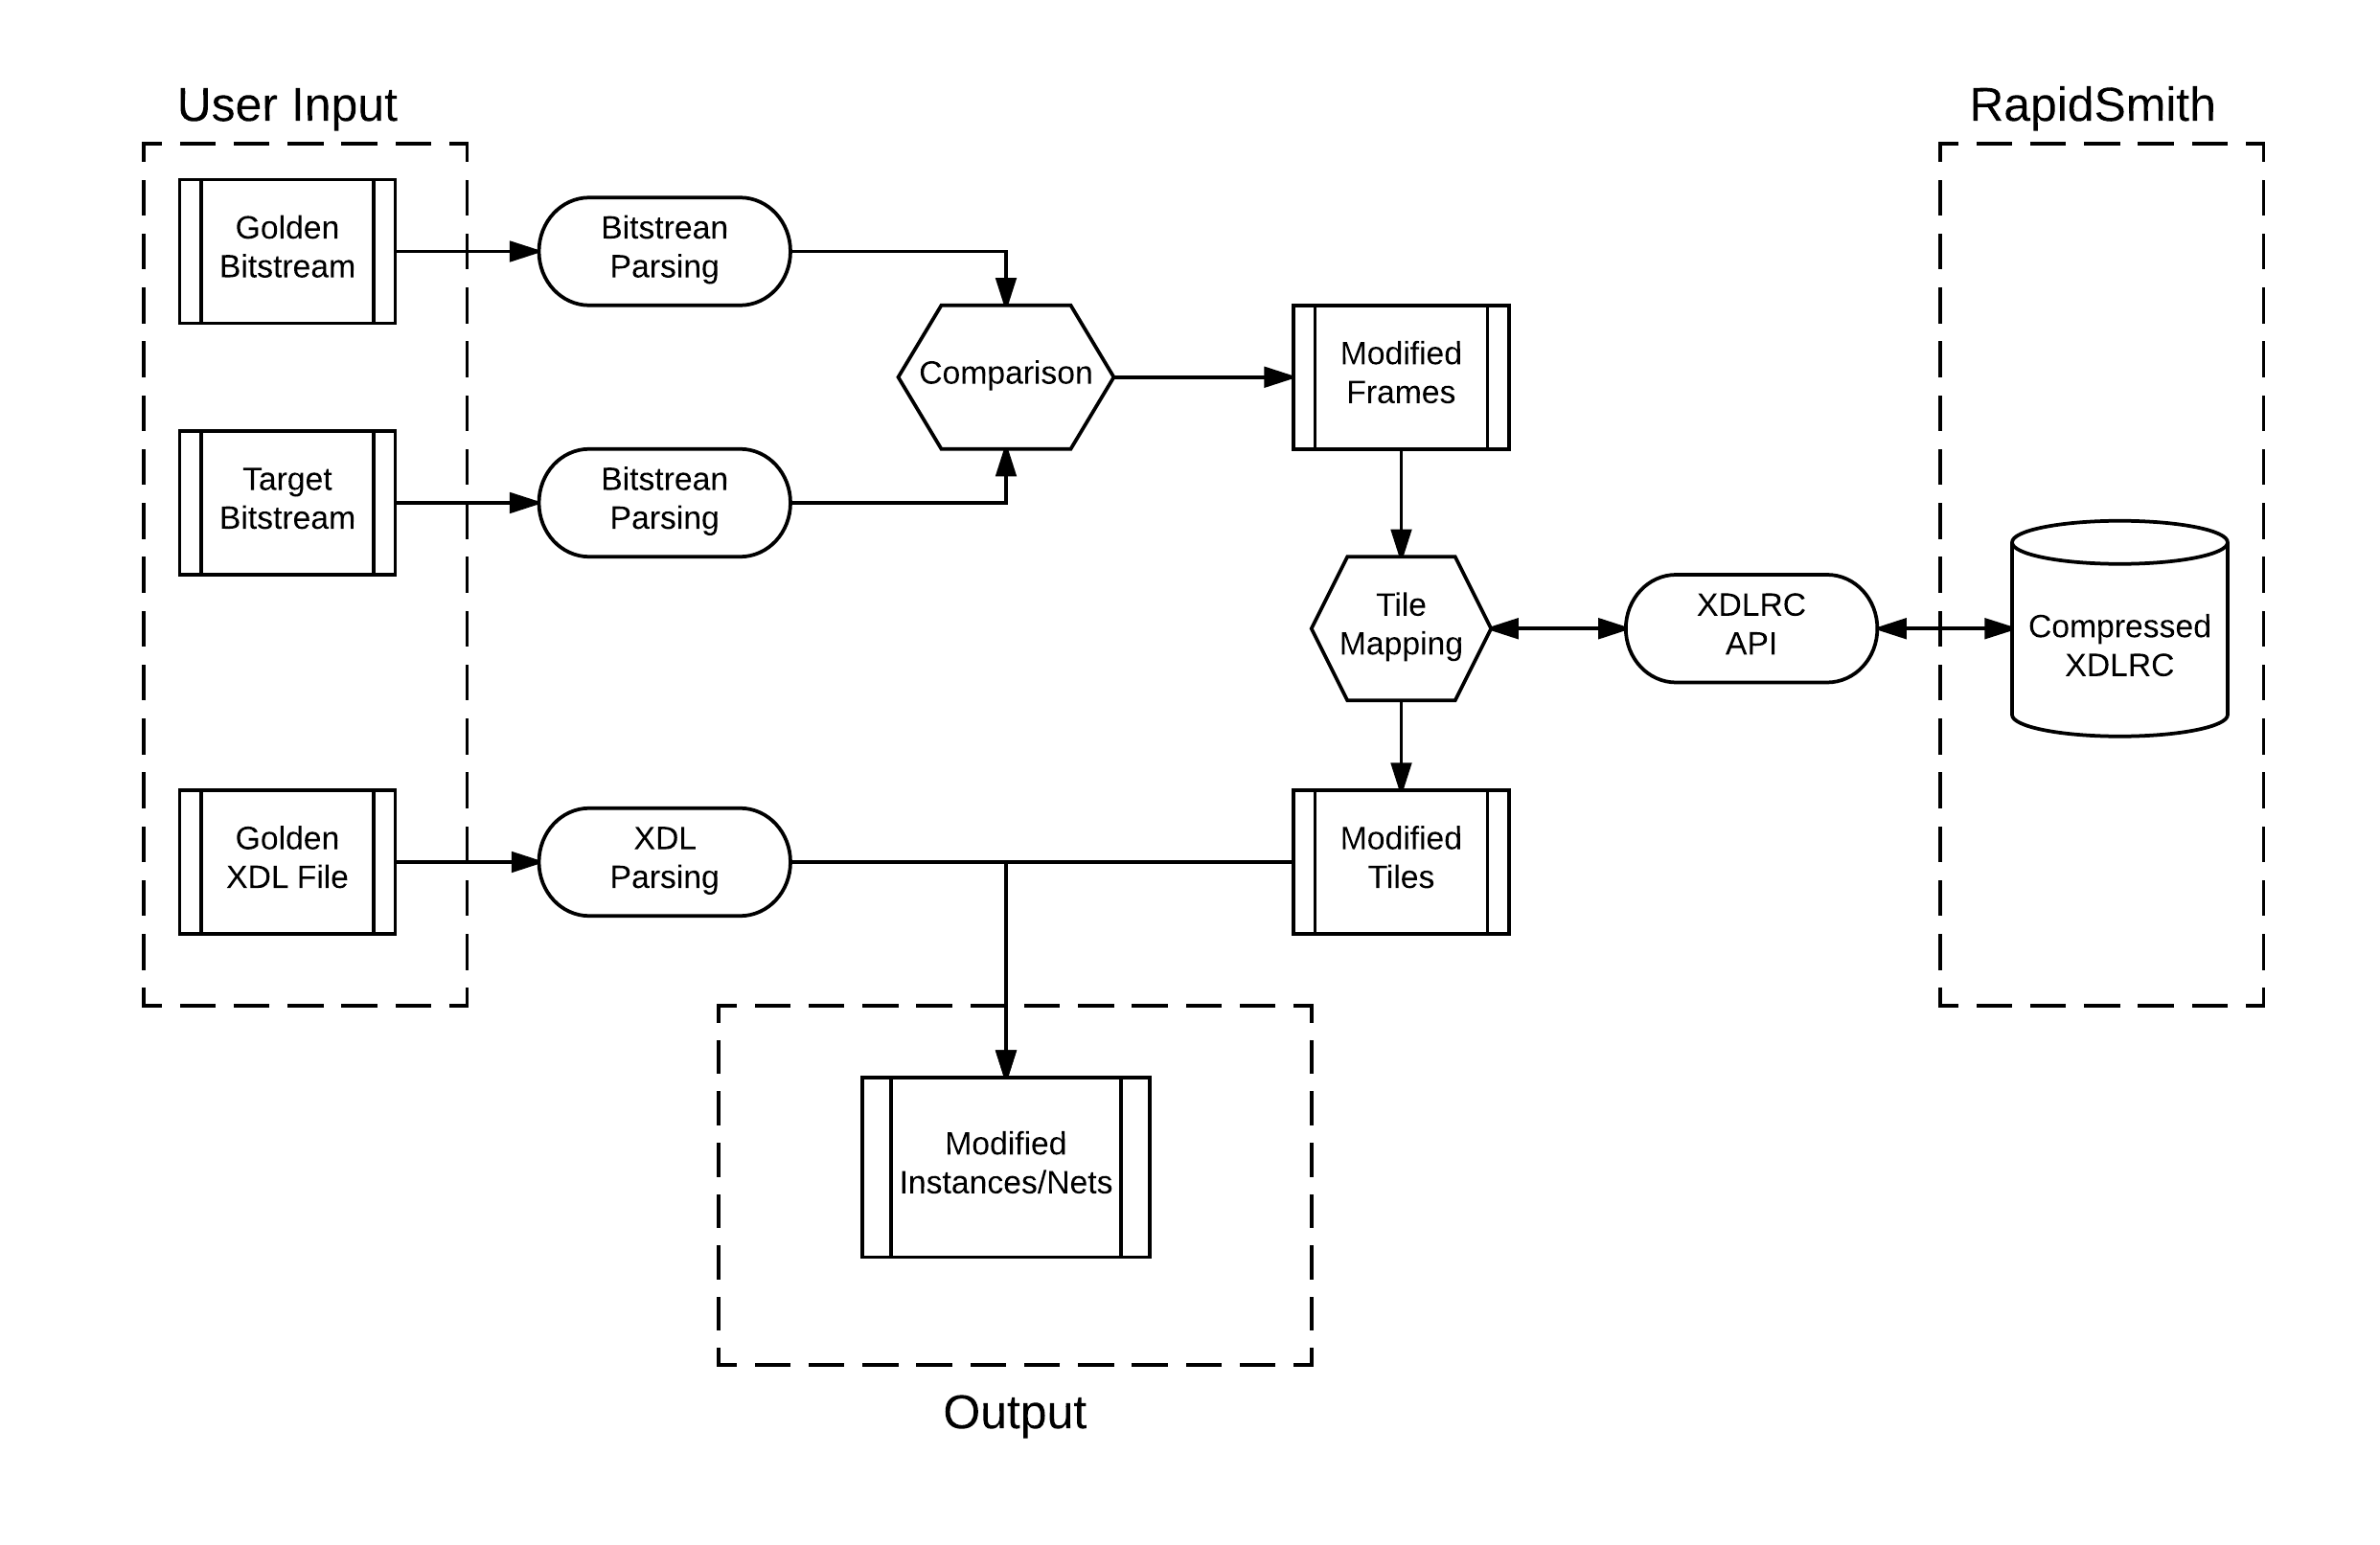
\includegraphics[width=1\linewidth]{Figures/Operation}
	\caption[Overview of Functional Operation]{Overview of Functional Operation}
	\label{fig:Operation}
\end{figure}

Knowing the device, the parser is able to refer to additional utility files and accurately extract the frames.
The \gls{golden} and \gls{target} frames are extracted and stored in memory as arrays.
The two arrays are then passed to a comparison process.
Each frame is compared bit by bit.
A trojan-free circuit will have no differences between the \gls{golden} and \gls{target} files.
Any modified frames discovered are stored in a 'Modified\_Frame' class.
The 'Modified\_Frame' object stores the \gls{golden} frame data, the \gls{target} frame data, the address of the frame and more.
They are then used by the 'Component Mapping' method described in section~\ref{sec:tileMapping} to determine where in the architecture the modifications have been made.

The component mapping procedure relies heavily on the compressed XDLRC files and the corresponding \acrshort{API} described in section~\ref{sec:XDLRC} as well as the 'Device' class structure shown in Figure~\ref{fig:rapidSmithDevice}.
Component mapping produces a list of objects of the 'Modified\_Tile' class.
This class contains a reference to the corresponding tile in the XDLRC file, the \gls{golden} and \gls{target} words (which differ), the frame address in which it occurred, the sub-column type and the column type.
The user is also required to enter the \gls{golden} \acrshort{XDL} file.
As described in section~\ref{sec:XDL} the \acrshort{XDL} file contains the Netlist for the \gls{golden} design.
This file describes not only how each of the users components are built and interconnected but where on the device they are placed.
The modified tiles, as shown in Figure~\ref{fig:Operation}, must be correlated to the users design to extract useful information.
The instances and nets described in the \acrshort{XDL} file list the exact tile and primitive in which they are placed.
The \RapidSmith \acrshort{XDL} parser reads the user's design and populates the 'Design' class shown in Figure~\ref{fig:rapidSmithDesign}.
The list of 'Modified\_Tile' objects are compared to the tile placings of the instances and nets in the populated 'Design' object.
Any instances or nets that are placed in 'modified' tiles are flagged and stored.
The user is able to view which instances and nets of their design have been modified by the four buttons on the right of the \acrshort{UI} shown in Figure~\ref{fig:UI}.
\subsection{The Web Environment} \label{sec:webEnvironment}
The HTS was designed as a web utility for portability and easy distribution.
The application server performs all of the computations and generates page markup to minimize the burden on client-side browsers.
It communicates directly with a remote database used to store user account information and application data (attributes, categories and matrices).
Both the application server and the database are hosted on the Microsoft Azure Cloud platform~\cite{Azure}.
This improves reliability, portability, and flexibility, provides on-demand resources that are automatically managed for scalability requirements,
and allows for maintenance to take place anywhere.
Fig.~\ref{fig:TrojanDistribution} gives a block diagram of the HTS.
%\color{red}
The application server and database are both hosted on the Azure Cloud~\cite{Azure}.
The entity framework provides communication via efficient and secure SQL statements while
Azure provides dynamic resource allocation.
When the system is not being used, the architecture is stored in memory to reduce costs.
When a client browser attempts to connect to the system, the application server and database are re-activated.
Requests and responses are passed between the client side browsers and application server via JavaScript Object Notation (JSON) strings.
This allows for complex object oriented logic to be processed across the network in a simple and efficient manner.
%\color{black}
\begin{figure}[h]
	\centering
	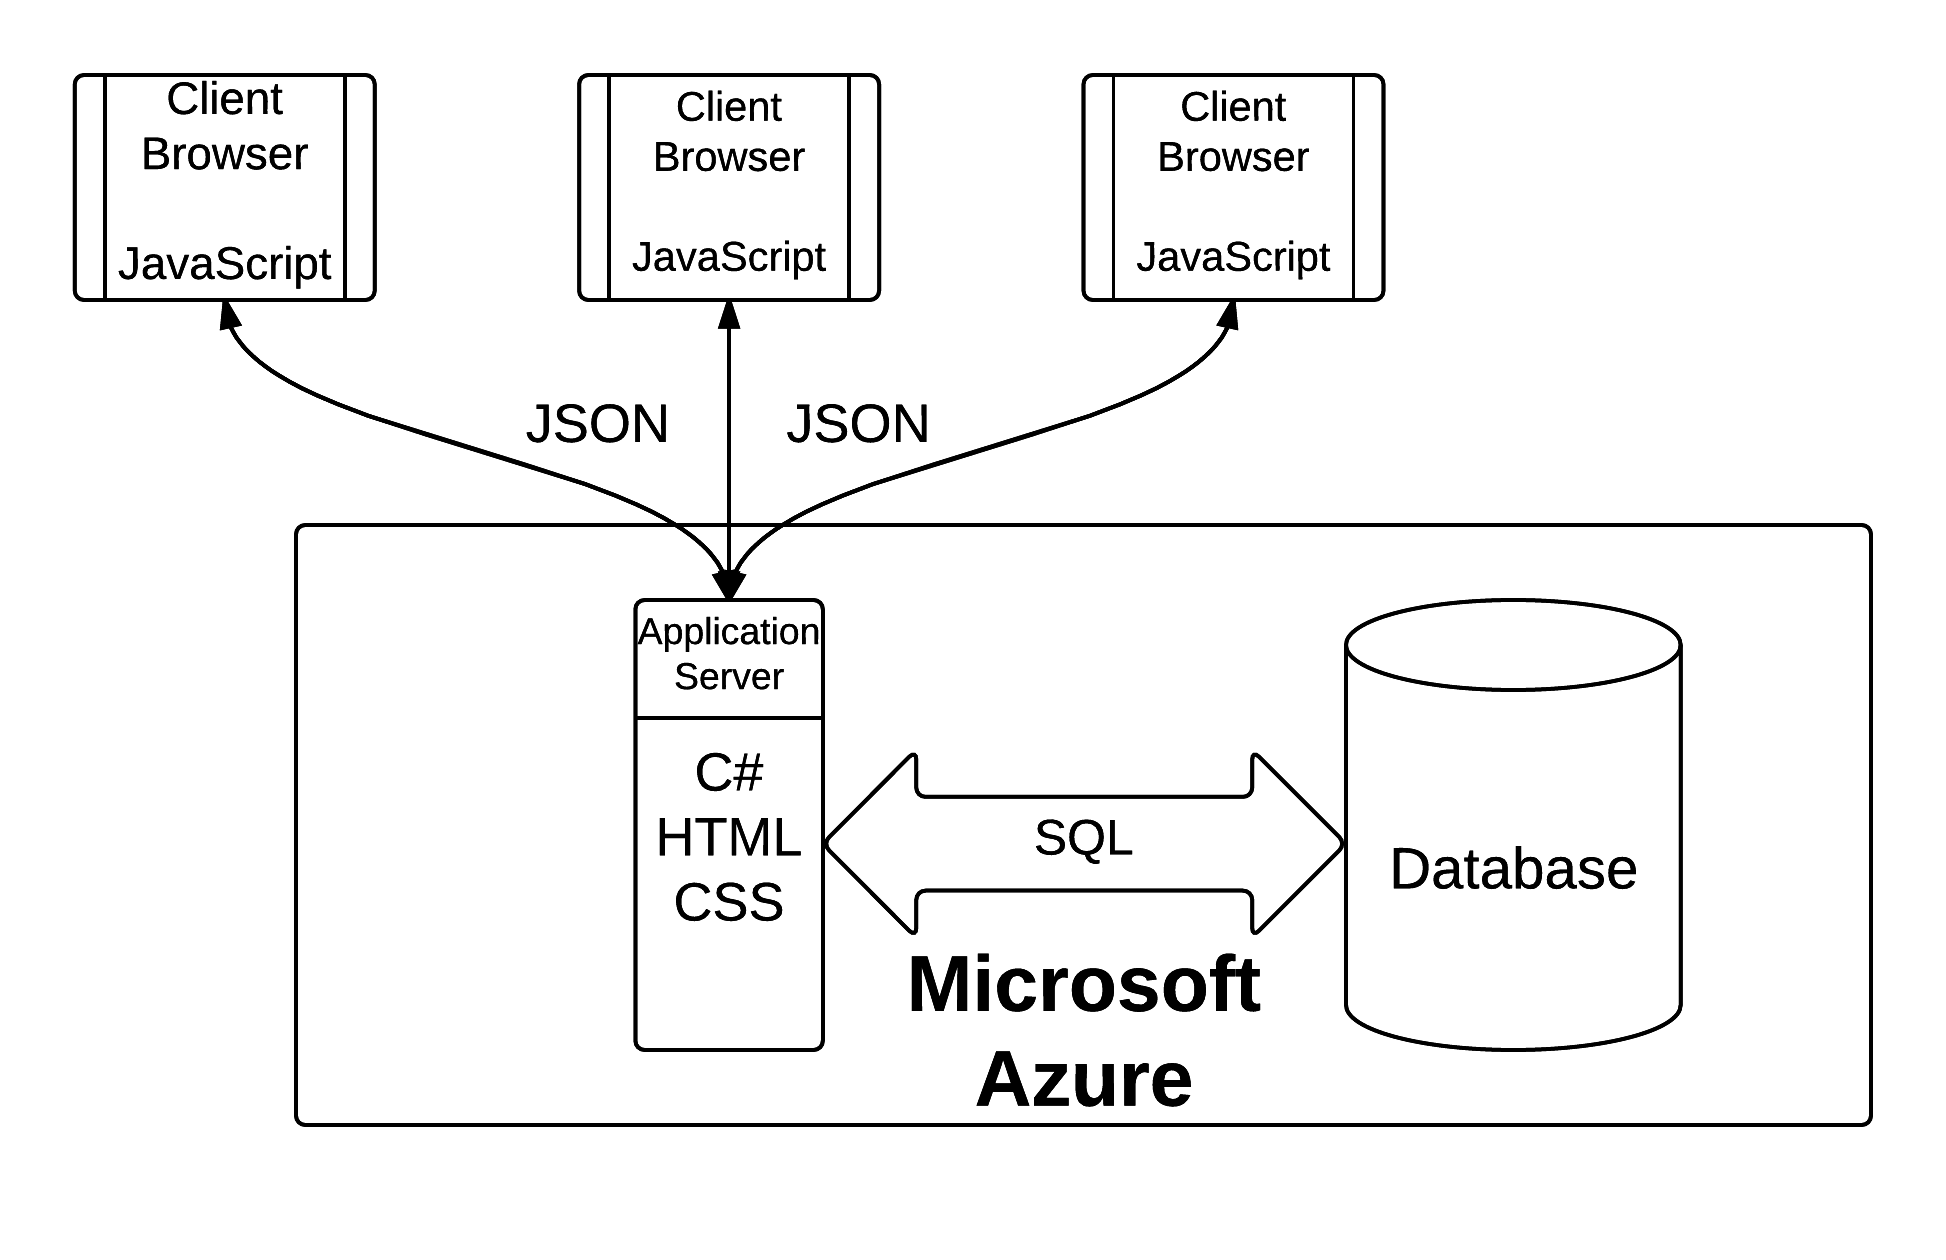
\includegraphics[height = 7cm]{figures/Distribution}
	\caption{Block diagram of the hardware trojan system (HTS).}
	\label{fig:TrojanDistribution}
\end{figure}

The technologies employed are as follows.
\begin{itemize}
	\item \textbf{Azure:} The Microsoft cloud system \cite{Azure}.
	\item \textbf{ASP.NET Web Form:} A user interface focused, event-driven model of the .NET framework.
	It allows powerful data-binding, separation of server-client side activities, a native security structure, and enhanced client performance \cite{ASP}.
	\item \textbf{Entity Framework:} An object-relational database mapper designed for the .NET framework.
	It provides a library of high speed SQL statements wrapped in C\# commands to simplify development and ensure performance \cite{Entity}.
	\item \textbf{D3.js:} A Java-script library for visualizing data with HTML, SVG and CSS \cite{D3}.
\end{itemize}
Fig.~\ref{fig:WebsiteArchitecture} provides an overview of the structure of the HTS website.
The \textit{home, contact}, \textit{about}, and \textit{application information} pages are accessible to all traffic.
The application information page contains three sub-pages providing information on each of the primary applications.
Users are required to create an account and be logged in to access the remainder of the website.
Email confirmation is used to verify user accounts.
\begin{figure}[h]
	\centering
	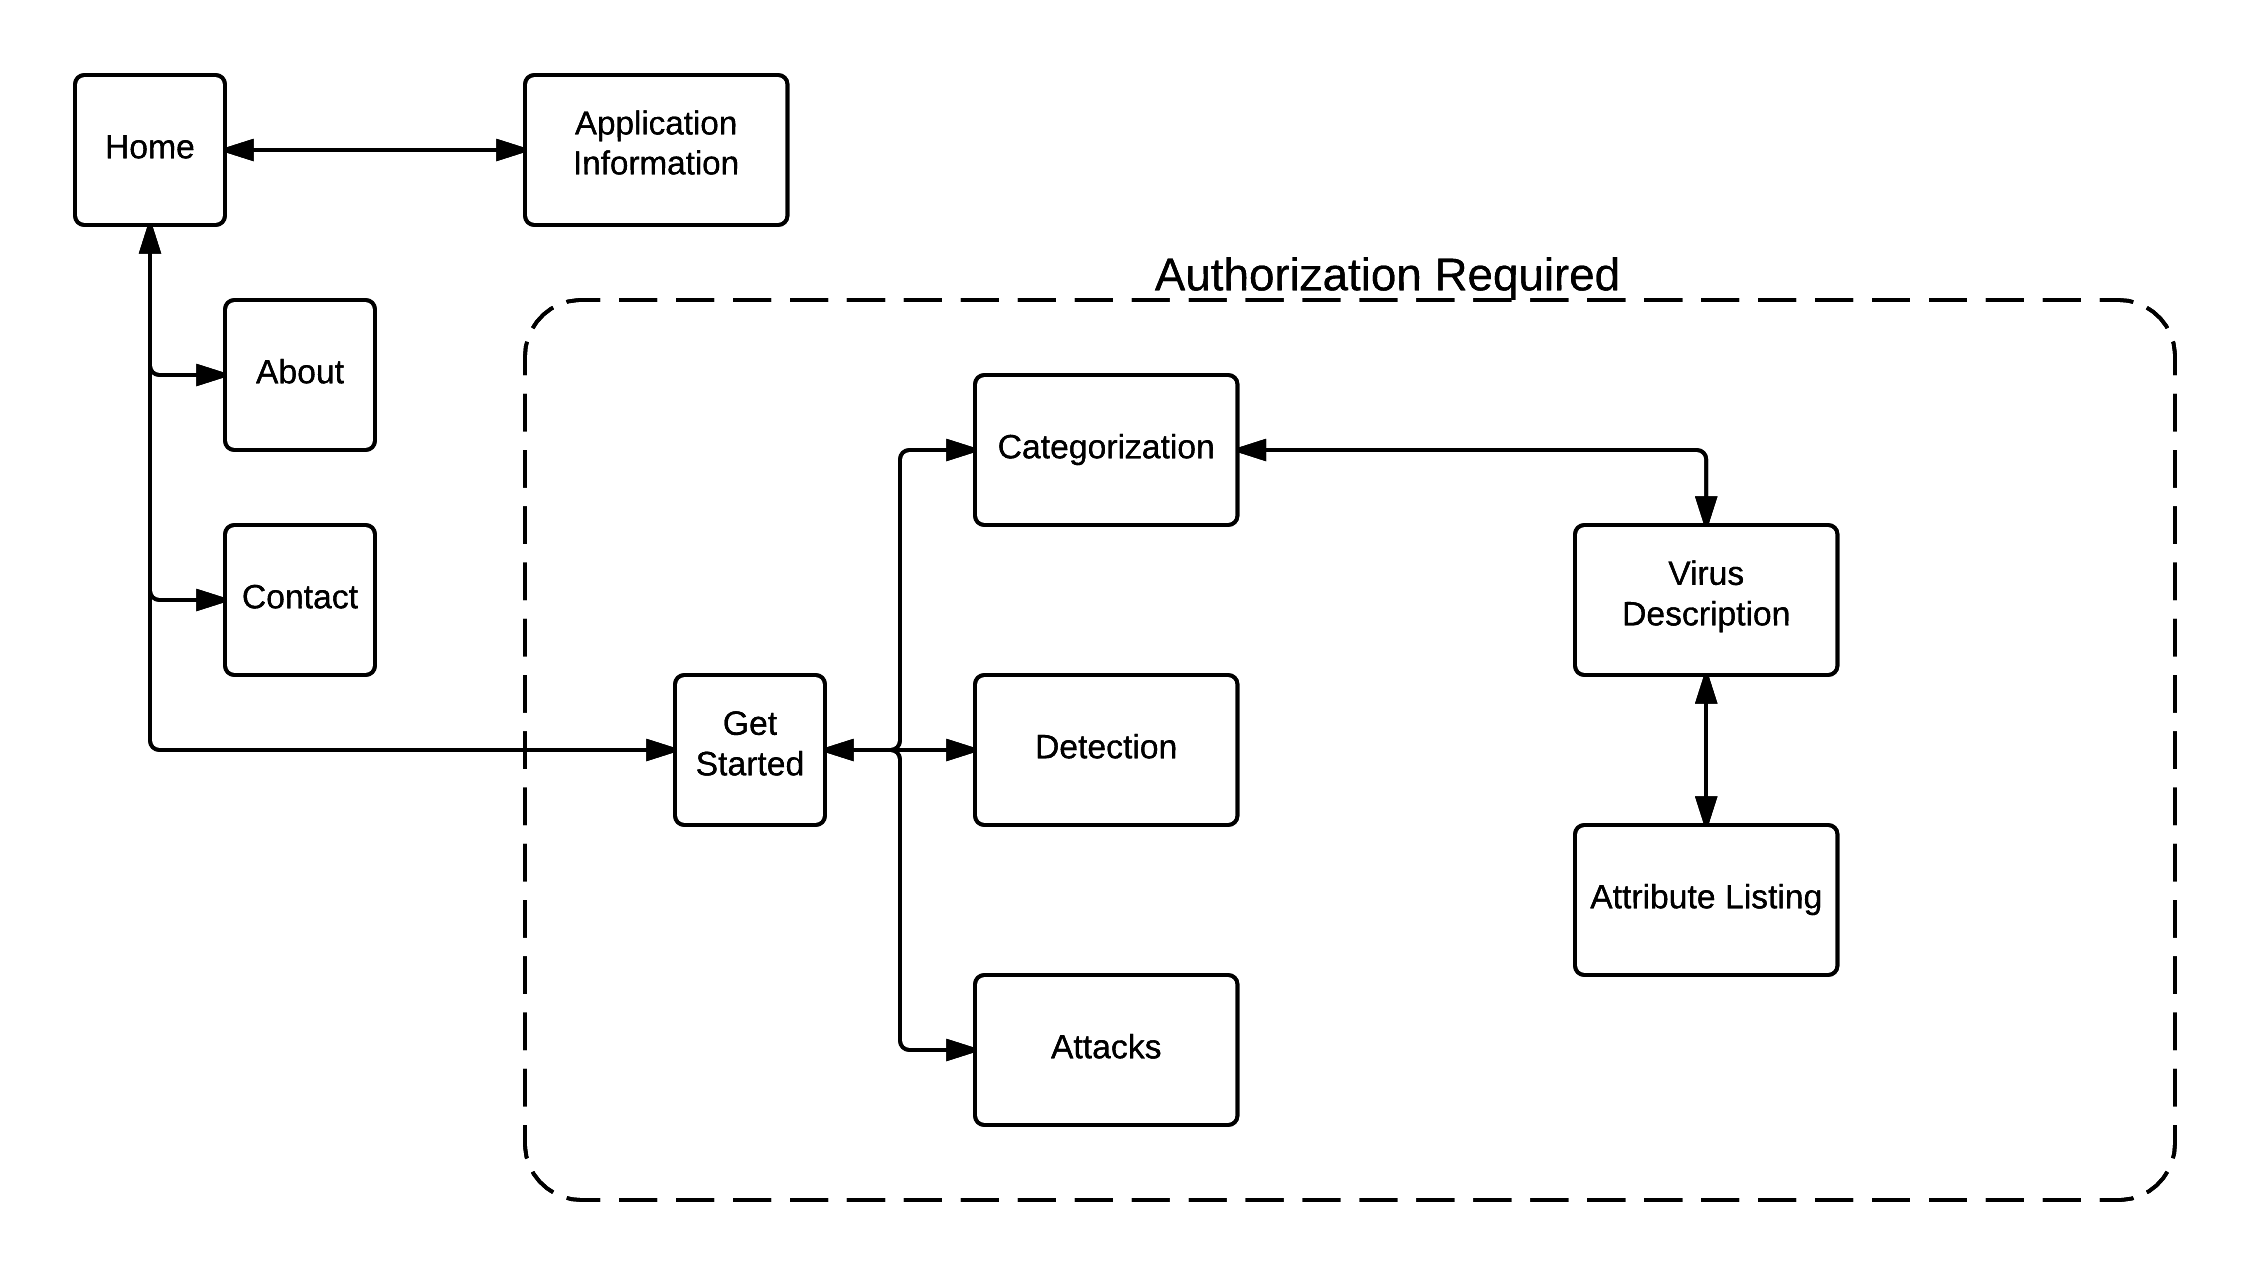
\includegraphics[height = 7cm]{figures/WebsiteArchitecture}
	\caption{An overview of the website architecture.}
	\label{fig:WebsiteArchitecture}
\end{figure}

%This is a good place to put tables, lots of results, perhaps all the data compiled in the experiments. By avoiding putting all the results inside the chapters themselves, the whole thing may become much more readable and the various tables can be linked to appropriately.
%
%The main purpose of an Appendix however should be to take care of the future readers and researchers. This implies listing all the housekeeping facts needed to continue the research. For example: where is the raw data stored? where is the software used? which version of which operating system or library or experimental equipment was used and where can it be accessed again?
%
%Ask yourself: if you were given this thesis to read with the goal that you will be expanding the research presented here, what would you like to have as housekeeping information and what do you need? Be kind to the future graduate students and to your supervisor who will be the one stuck in the middle trying to find where all the stuff was left!



% The style of bibliography exemplified here is the "plain",
% normally used in science theses. This is shown
% by the entry {plain} below. Substitute the
% appropriate bibliography style. See also the
% PDF file "InformationOnBibliographyStyles" in this
% directory for more choices.

% The Bibliography file is a BibTex file named
% UVicThesis.bib and called below

	\TOCadd{Bibliography}
	\bibliographystyle{plain}
	%\bibliographystyle{./IEEEtran}
	\bibliography{UvicThesis}

\end{document}
